\documentclass[hidelinks,12pt]{article}
\usepackage{graphicx}
\usepackage{layout}
\usepackage{amsmath, amssymb}
\usepackage{hyperref}
\usepackage{float}
\usepackage{fancyhdr}
\usepackage{titlesec}
\usepackage[dvipsnames]{xcolor}
\usepackage{lipsum}
\usepackage{cleveref}
\usepackage[a4paper,left=3cm,right=2cm,top=2.5cm,bottom=2.5cm]{geometry}
\usepackage{overpic}
\usepackage{booktabs}
\usepackage{subcaption}
\usepackage{titlesec}
\usepackage{caption}
\usepackage{lipsum}
\usepackage{enumitem}

\pagestyle{fancy}
\fancyhf{}
% \renewcommand{\headrulewidth}{0pt}
\cfoot{\thepage}

\setlength{\parindent}{0pt}

\author{M.M. Roshani}

\begin{document}
	\begin{titlepage}
		\begin{center}
			
\includegraphics[width=10cm]{figures/SUT_logo.png} \\
			\vspace{1cm}
			\textbf{\Large ENGINEERING MATHEMATICS PROJECT}\\
			\vspace{0.5cm}
			Instructor: Prof. Hamid Aghajan\\
			\vspace{1cm}
			\textbf{\Large SHARIF UNIVERSITY OF TECHNOLOGY}\\
			\vspace{1cm}
			\rule{\linewidth}{0.5mm} \\
			\vspace{0.5cm}
			{\Huge \textbf{From Noise to Clarity:}}\\
			\vspace{0.3cm}
			{\huge \textbf{A Study of Filtering Techniques in}}\\
			\vspace{0.3cm}
			{\huge \textbf{Biomedical Imaging}}\\
			\rule{\linewidth}{0.5mm} \\
			\vfill
			\textbf{\Large M.M. Roshani}
		\end{center}
	\end{titlepage}
	
	\tableofcontents
	\newpage
	
	\section{Aspects of an Image}
	
	Using Figure~\textcolor{Cyan}{\ref{fig:kobe}} answer the following questions: \\
	
	\textbf{1.} Intuitively, What do low and high frequencies of an arbitrary image contain? Which
	one is more important? Do you think your answer depends on the image? Explain it.
	\\ \\
	 Intuitively, high-frequency components represent sudden changes in an image, such as edges or details. We humans can detect objects based on high frequencies. On the other hand, low frequencies correspond to smooth changes or uniform areas of an image. For instance, in fingerprints, high frequencies are more important. Because without them, it would be impossible to see the outlines of ridges. Conversely, in images with gradual transitions, like landscapes, lower frequencies can give us more information. Therefore, determining which one is more important depends on the context.
	
	\vspace*{2\baselineskip}
	 \textbf{2.} Explain about low pass filter(LPF) and high pass filter(HPF). In what applications LPF and HPF are used? Write two functions that apply LPF and HPF to an arbitrary image.
	
	
	\begin{figure}[b!]
		\centering
		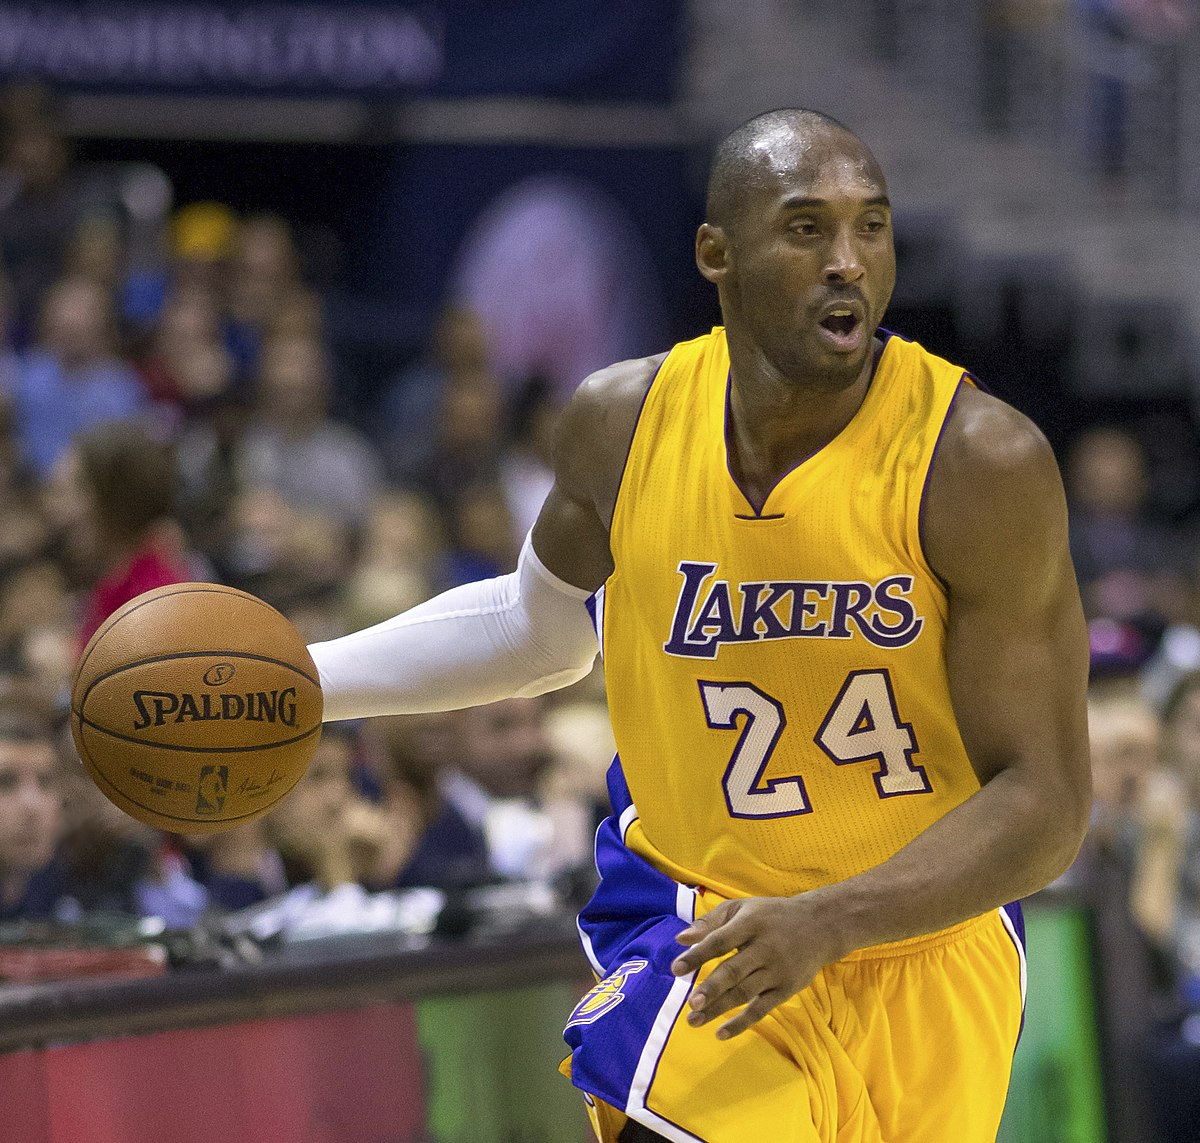
\includegraphics[scale=0.28]{figures/pic1.jpg}
		\caption{Kobe Bryant (August 23, 1978– January 26, 2020)}
		\label{fig:kobe}
	\end{figure}
	
	\pagebreak
	
	 A Low-Pass Filter (LPF) allows signals with frequencies lower than a certain cutoff frequency to pass through while diminishing higher frequencies. On the other hand, a High-Pass Filter (HPF) allows signals with frequencies higher than a cutoff frequency to pass while attenuating lower frequencies. Let's look at two applications of each filter.
	
	\begin{itemize}
		\item \textbf{Audio Processing:} LPFs remove high-frequency noise and hiss, making speech and music smoother, commonly used in hearing aids and audio mixing. HPFs eliminate low-frequency disturbances like wind noise, mic handling noise, and electrical hum, improving clarity in recordings and live audio.
		
		\item \textbf{Image Processing:} LPFs blur images to reduce noise and smooth details, useful in artifact reduction. They are also used in image compression by removing high-frequency details before quantization, reducing data complexity and improving compression efficiency. HPFs enhance edges and fine details, aiding in sharpening, edge detection, and applications like medical imaging and fingerprint recognition.
	\end{itemize}
	
	 Now we apply LPF and HPF to the image below.
	
	\begin{figure}[hb!]
		\centering
		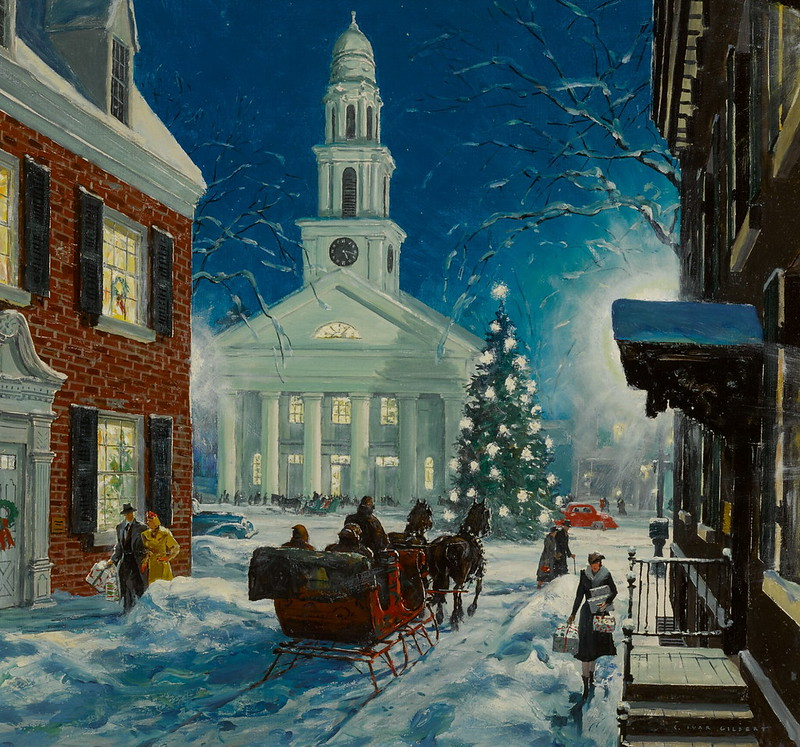
\includegraphics[scale=0.25]{figures/christmas_eve.jpg}
		\caption{CHRISTMAS EVE | CARL IVAR GILBERT}
	\end{figure}
	
	
	\begin{figure}[!h]
		\centering
		\begin{subfigure}{0.45\textwidth}
			\centering
			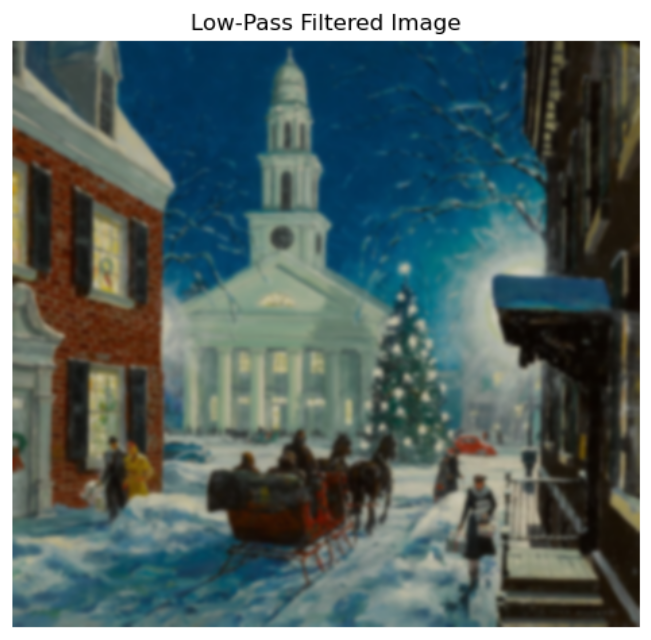
\includegraphics[width=\linewidth]{figures/christmas_eve_lpf.png}
		\end{subfigure}
		\hfill
		\begin{subfigure}{0.45\textwidth}
			\centering
			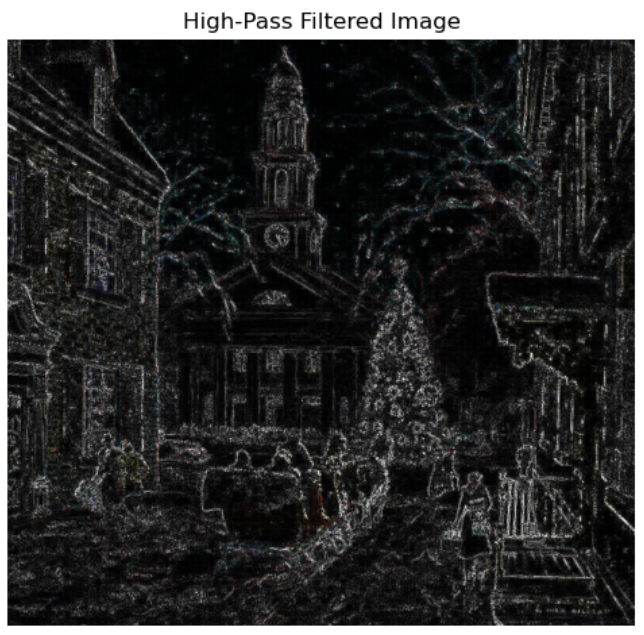
\includegraphics[width=\linewidth]{figures/christmas_eve_hpf.png}
		\end{subfigure}
	\end{figure}
	
	\pagebreak
	
	 \textbf{3.} Apply LPF and HPF to Figure~\textcolor{Cyan}{\ref{fig:kobe}} using functions written in the previous part. Explain	the results.
	
	\begin{figure}[hb!]
		\centering
		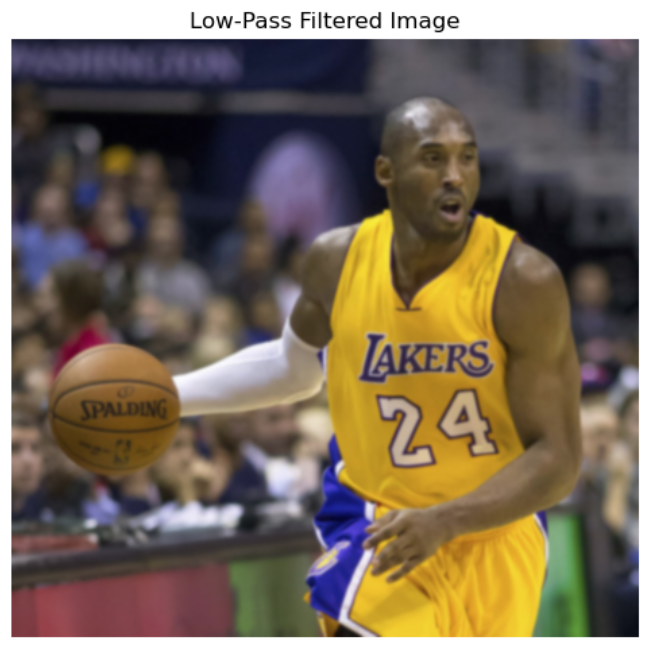
\includegraphics[scale=0.62]{figures/kobe_lpf.png}
	\end{figure}
	
	\begin{figure}[hb!]
		\centering
		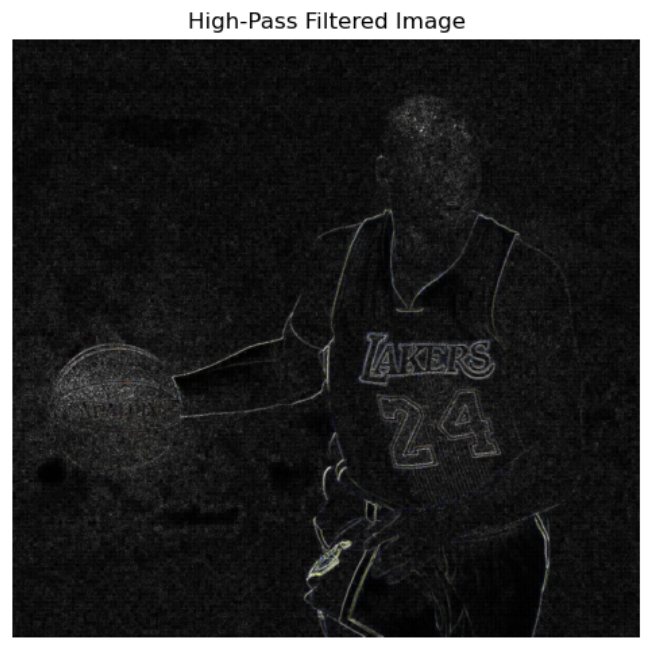
\includegraphics[scale=0.62]{figures/kobe_hpf.png}
	\end{figure}
	
	
	  In the top image, the player's jersey, face, and overall shape are smooth, but details like the jersey's text edges and facial features are less apparent. In the bottom, the edges of the player's jersey, the ball, and facial features are visible, while flat regions (like the background and smooth surfaces) are darkened. As expected, applying an LPF makes the image blurry and results in a loss of detail. On the other hand, an HPF enhances edges and brings out finer details.
	
	\pagebreak
	
	
	 Using Figure~\textcolor{Cyan}{\ref{fig:pic2}} and Figure~\textcolor{Cyan}{\ref{fig:pic3}} answer questions below.
	
	
	\begin{figure}[h]
		\centering
		\begin{subfigure}{0.45\textwidth}
			\centering
			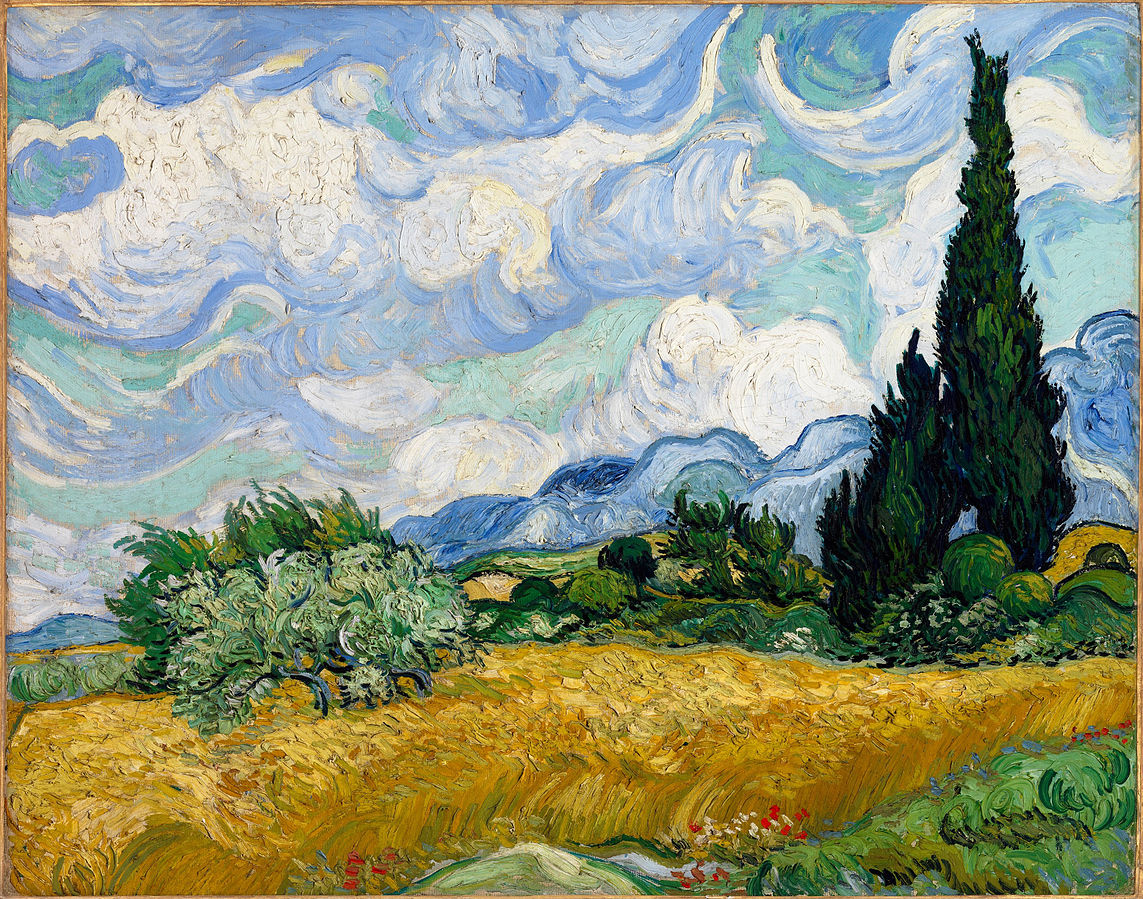
\includegraphics[width=\linewidth]{figures/pic2.jpg}
			\caption{Wheat Field with Cypresses}
			\label{fig:pic2}
		\end{subfigure}
		\hfill
		\begin{subfigure}{0.45\textwidth}
			\centering
			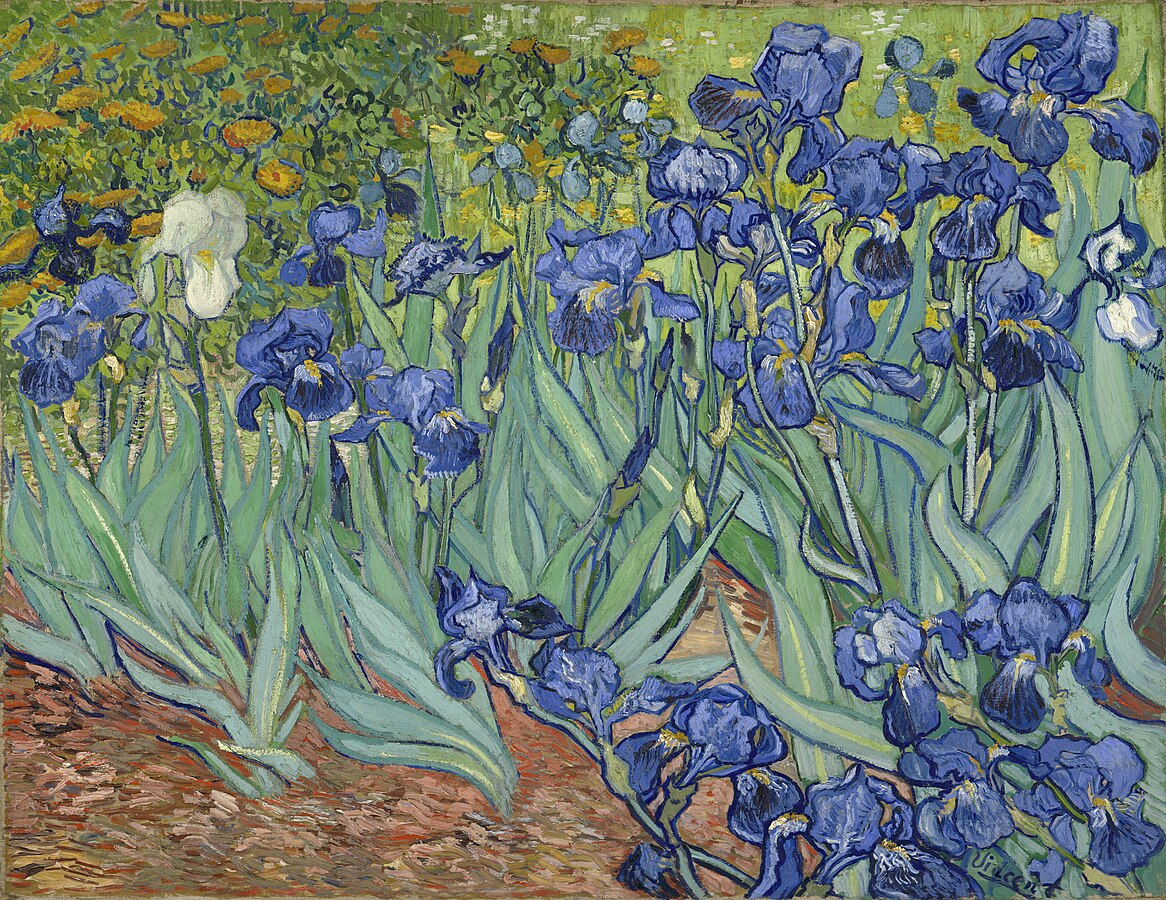
\includegraphics[width=\linewidth]{figures/pic3.jpg}
			\caption{Irises}
			\label{fig:pic3}
		\end{subfigure}
	\end{figure}
	
	
	 \textbf{4.} Plot the magnitude and phase of both images. Then, plot an image with magnitude of Figure~\ref{fig:pic2} and phase of Figure~\ref{fig:pic3}. Plot the other alternate.
	
	\begin{figure}[h!]
		\centering
		\begin{subfigure}[b]{0.45\textwidth}
			\centering
			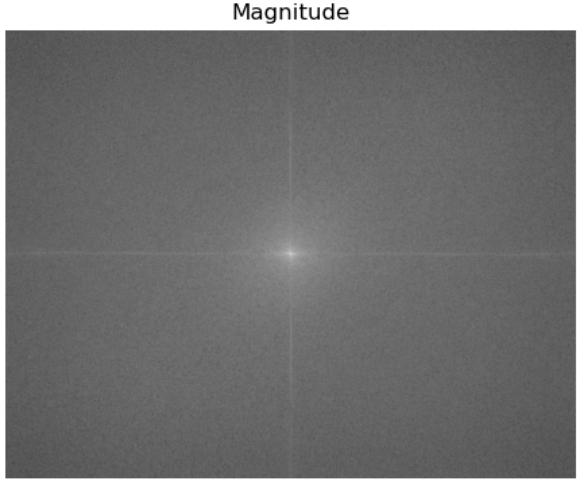
\includegraphics[width=\textwidth]{figures/pic2_mag.PNG}
		\end{subfigure}
		\hspace{0.5cm}
		\begin{subfigure}[b]{0.45\textwidth}
			\centering
			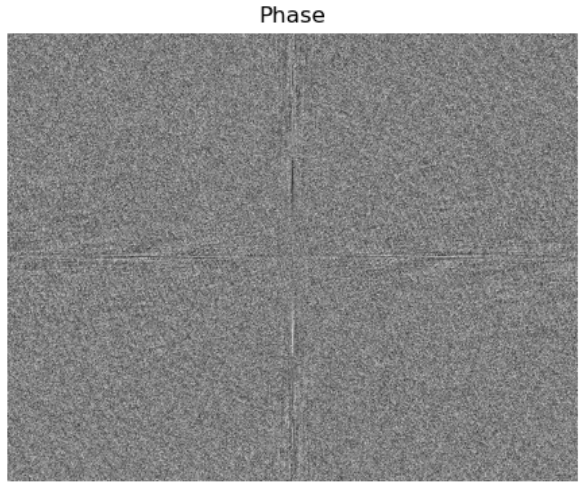
\includegraphics[width=\textwidth]{figures/pic2_phase.PNG}
		\end{subfigure}
		\caption{Magnitude and phase plot of Figure~\ref{fig:pic2}}
	\end{figure}
	
	\begin{figure}[h!]
		\centering
		\begin{subfigure}[b]{0.45\textwidth}
			\centering
			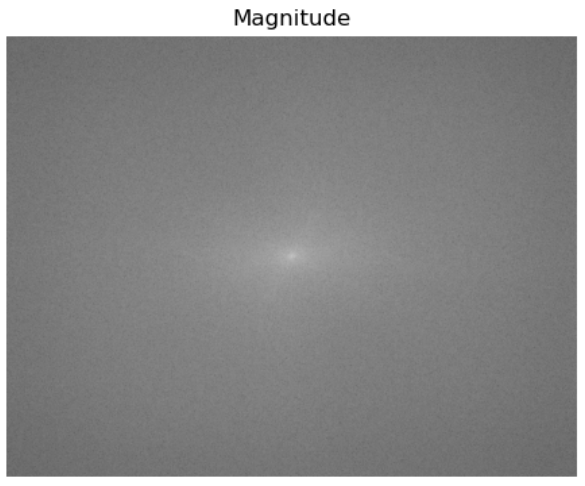
\includegraphics[width=\textwidth]{figures/pic3_mag.PNG}
		\end{subfigure}
		\hspace{0.5cm}
		\begin{subfigure}[b]{0.45\textwidth}
			\centering
			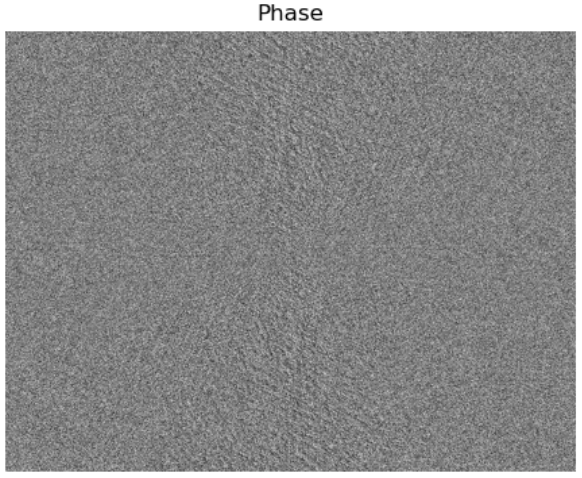
\includegraphics[width=\textwidth]{figures/pic3_phase.PNG}
		\end{subfigure}
		\caption{Magnitude and phase plot of Figure~\ref{fig:pic3}}
	\end{figure}
	
	\pagebreak
	
	\begin{figure}[!h]
		\centering
		\begin{tabular}{c}
			\begin{subfigure}[h]{0.45\textwidth}
				\centering
				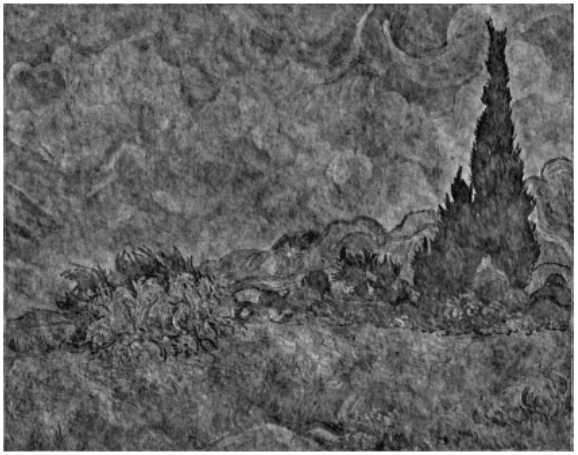
\includegraphics[width=\textwidth]{figures/mag3_phase2.PNG}
			\end{subfigure}
			\hfill
			\begin{subfigure}[h]{0.45\textwidth}
				\centering
				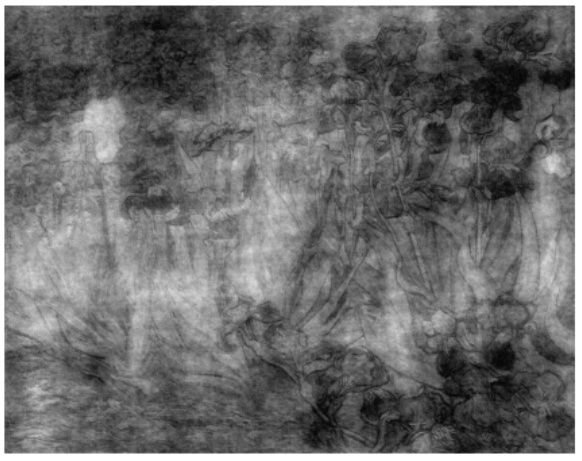
\includegraphics[width=\textwidth]{figures/mag2_phase3.PNG}
			\end{subfigure} \\
			
			\begin{subfigure}[h]{0.45\textwidth}
				\centering
				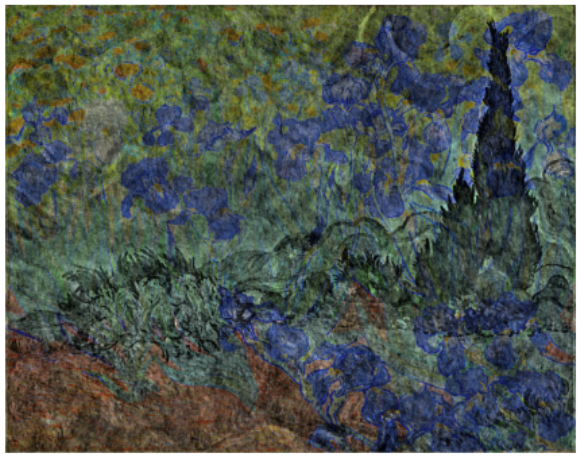
\includegraphics[width=\textwidth]{figures/mag3_phase2_color.PNG}
				\caption{Magnitude Fig.~\ref{fig:pic3} + Phase Fig.~\ref{fig:pic2}}
			\end{subfigure}
			\hfill
			\begin{subfigure}[h]{0.45\textwidth}
				\centering
				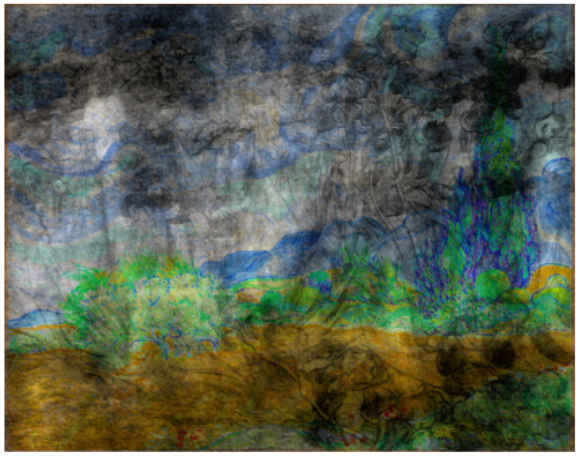
\includegraphics[width=\textwidth]{figures/mag2_phase3_color.PNG}
				\caption{Magnitude Fig.~\ref{fig:pic2} + Phase Fig.~\ref{fig:pic3}}
			\end{subfigure}
		\end{tabular}
		\caption{}
		\label{fig:mixed_phase_mag}
	\end{figure}
	
	 \textbf{5.} Using the results above, Explain Why is the phase information more critical for reconstructing recognizable features of an image compared to the magnitude information?
	
	
	\paragraph{}
	If we compare Figure~\ref{fig:mixed_phase_mag} with the original images, we can see that the images with the same phase look similar. That is because the phase information plays a critical role in reconstructing recognizable features of an image. It determines the spatial arrangement of the image's frequency components. While the magnitude provides the strength or amplitude of each frequency, it does not convey how these frequencies are arranged in space. The phase information, however, controls the placement of edges and shapes in an image, which are key to its structure.
	
	\paragraph{}
	When the phase is altered, even if the magnitude remains intact, the image loses its structure. This results in a blurred or distorted image that lacks recognizable features. Although the intensity (magnitude) might still be visible in some form, the critical spatial relationships that define the image are missing.
	
	\paragraph{}
	In contrast, removing the magnitude while preserving the phase leads to a loss of intensity and sharpness, but the image's overall structure can still be detected. This shows that phase information is more important for the spatial arrangement of features, whereas magnitude primarily influences the contrast and brightness of the image.
	
	
	\pagebreak
	
	\section{Noise}
	\subsection{Questions}
	
	 \textbf{1.} What are the primary sources of salt-and-pepper noise in digital images, and what filtering techniques are most effective in mitigating this type of noise?
	\\ \\
	Salt-and-pepper noise, characterized by random white (salt) and black (pepper) pixels, is a type of impulse noise that can degrade the quality of digital images. The primary sources of salt-and-pepper noise are:
	\begin{itemize}
		\item \textbf{Sensor Malfunctions}: Faulty sensors or detectors in digital cameras or imaging devices can cause random bright or dark pixels in the captured image.
		\item \textbf{Transmission Errors}: During data transmission (such as when sending images over a network), errors or corruption in the data stream can lead to random pixel values being replaced.
		\item \textbf{Environmental Factors}: Low-quality or malfunctioning hardware, such as old or poorly maintained imaging devices, can also introduce noise. Electromagnetic interference or poor lighting conditions can also worsen these issues.
	\end{itemize}
	
	 \textbf{Effective Filtering Techniques:} Two of the most common filtering techniques are:
	
	\begin{itemize}
		\item \textbf{Median Filtering}
		
		Median filtering is the most commonly used and effective method for salt-and-pepper noise. It works by replacing each pixel value with the median value of its neighboring pixels within a defined window (e.g., a 3x3 or 5x5 window). The median filter is particularly effective because it is good at preserving edges while removing the extreme values (salt and pepper).
		
		\item \textbf{Adaptive Filters}
		
		Adaptive filtering techniques, such as adaptive median filtering, adjust the size of the filtering window based on local characteristics of the image (e.g., noise density). These filters can adapt to different noise levels and are particularly useful when the noise density varies across the image.
		
		
	\end{itemize}
	
	
	 \textbf{2.} How does electrical interference introduce 50Hz noise into signal recordings, and what methods can be employed to eliminate or reduce this interference?
	\\ \\
	Electrical interference often arises from the power supply grid, which in many regions operates at a frequency of 50Hz (or 60Hz in some countries). This can introduce periodic noise at the same frequency (50Hz) into signal recordings, especially in environments with sensitive electronic equipment like audio, video, or biomedical signal recording devices.
	
	\pagebreak
	
	 The primary causes of this interference include:
	
	\begin{itemize}
		\item \textbf{Coupling from Power Lines}: Electrical systems, especially AC power lines, emit electromagnetic fields that can couple with the cables and circuits of nearby recording equipment. The interference can enter the system through means such as direct contact, capacitive or inductive coupling.
		\item \textbf{Ground Loops}: Equipment connected to different ground points may experience a difference in electrical potential, creating a loop that picks up noise from the power supply.
		\item \textbf{Imperfect Shielding}: Cables and equipment that are not adequately shielded may act as antennas, picking up electromagnetic noise and introducing it into the signal.
	\end{itemize}
	
	
	 \textbf{Methods to Eliminate or Reduce 50Hz Noise}
	
	\begin{itemize}
		\item \textbf{Notch Filtering}: A notch filter is a type of band-stop filter that specifically targets and removes a narrow frequency band, such as the 50Hz noise. It suppresses the 50Hz component while allowing other frequencies in the signal to pass through unaffected. This method is highly effective when the 50Hz noise is isolated and does not overlap with important signal frequencies.
		\item \textbf{Low-Pass or High-Pass Filtering}: A low-pass filter (to remove higher frequency noise) or a high-pass filter (to remove low-frequency interference) can help eliminate certain portions of the signal that may contain 50Hz noise. However, this method is less specific than a notch filter and may accidentally remove important signal content.
	\end{itemize}
	
	
	
	 \textbf{3.} Identify the common sources of Gaussian noise in imaging systems and discuss the most suitable algorithms for its removal without significantly degrading image quality.
	
	
	Gaussian noise, often modeled as random variations in pixel values with a Gaussian distribution, is a common type of noise in imaging systems. The sources of Gaussian noise include:
	
	\begin{itemize}
		\item \textbf{Sensor Noise}: The most common source of Gaussian noise is the image sensor itself. Sensors, such as CCD (Charge-Coupled Device) or CMOS (Complementary Metal-Oxide-Semiconductor) sensors, can introduce noise due to thermal fluctuations, photon shot noise, or imperfections in the sensor circuitry.
		\item \textbf{Transmission Noise}: Noise can also be introduced during the transmission of the image data from the sensor to the processing unit. This could be due to interference, signal degradation, or errors in the communication channel, often contributing to Gaussian noise characteristics.
		\item \textbf{Quantization Noise}: When an image is digitized (e.g., from an analog signal to a digital format), quantization errors can introduce Gaussian noise. This happens when continuous pixel values are mapped to a discrete set of values, leading to small random variations around the true values.
		\item \textbf{Environmental Factors}: External factors like temperature and light conditions can also impact the sensor's performance, introducing random noise. For instance, high temperatures can increase thermal noise in the sensor, leading to Gaussian noise in the image.
	\end{itemize}
	
	 \textbf{Suitable Algorithms for Removal of Gaussian Noise}
	
	\begin{itemize}
		\item \textbf{Gaussian Blur (Linear Filtering)}: The Gaussian blur filter is a simple and commonly used method for reducing Gaussian noise. It works by convolving the image with a Gaussian kernel, which smooths the image and reduces high-frequency noise components. While effective at noise reduction, the downside is that it can blur fine details and edges in the image.
		\item \textbf{Wiener Filter}: The Wiener filter is an adaptive filtering technique that works well for Gaussian noise removal. Unlike simple linear filters, it adapts to local image characteristics by estimating the local mean and variance, and then applying a filter that minimizes the mean square error between the filtered image and the original. It is more effective than Gaussian blur for preserving image details while reducing noise because it adjusts the degree of smoothing based on the local noise variance. However, it requires prior knowledge of the noise characteristics.
	\end{itemize}
	
	 \textbf{4.} Explore SNR and PSNR. What roles do Signal-to-Noise Ratio (SNR) and Peak Signal-to-Noise Ratio (PSNR) play in evaluating the effectiveness of noise removal techniques in digital images? Compare and contrast the effectiveness of SNR and PSNR in different applications such as medical imaging, video compression, and wireless communications.
	\\ \\
	 Signal-to-Noise Ratio (SNR) and Peak Signal-to-Noise Ratio (PSNR) are commonly used metrics to evaluate the quality of signals, including digital images, and the effectiveness of noise removal techniques.
	\\ \\
	\textbf{SNR:} is a measure of the ratio between the desired signal and the background noise. It quantifies how much stronger the signal is compared to the noise. The signal-to-noise ratio of a random variable $S$ to random noise $N$ is:
	$$
	SNR = \frac{E[S^2]}{E[N^2]}
	$$
	
	 it is useful in quantifying the overall quality of an image after noise removal, where a higher SNR value suggests that the noise has been effectively reduced without significant loss of detail in the image.
	\\ \\
	\textbf{PSNR:} is a more specific metric often used in the context of image quality evaluation, particularly when comparing the original and processed (or denoised) images. PSNR is calculated based on the mean squared error (MSE) between the original image and the denoised image. Given a noise-free m×n monochrome image I and its noisy approximation K, MSE is defined as:
	$$
	MSE = \frac{1}{mn} \sum_{i=0}^{m-1} \sum_{j=0}^{n-1} [I(i,j) - K(i,j)]^2
	$$
	$$
	PSNR = 10 \log_{10}(\frac{MAX_I^2}{MSE})
	$$
	
	 where $MAX_I$ is the maximum possible pixel value of the image. PSNR is sensitive to pixel-level changes, making it useful for applications where maintaining visual quality is crucial. In contrast, SNR reflects overall signal clarity, explaining why adaptive filters may show lower PSNR despite better visual quality., such as in image compression or denoising tasks.
	\pagebreak
	
	 \textbf{Comparison in Different Applications}
	\begin{itemize}
		\item \textbf{Medical Imaging}: SNR is crucial for ensuring that the signal (e.g., clinical details in an MRI or CT scan) is distinguishable from the noise. PSNR is used to evaluate the quality of processed medical images after denoising or compression, ensuring minimal loss of crucial information.
		\item \textbf{Video Compression}: PSNR is the preferred metric because it directly assesses the pixel-level quality after compression. SNR is less commonly used in this context, but may be relevant for assessing transmission quality.
		\item \textbf{Wireless Communications}: SNR is the key metric here, as it measures the strength of the received signal relative to noise, affecting the clarity and successful decoding of the signal. PSNR is not used in wireless communication.
	\end{itemize}
	
	 In summary, \textbf{SNR} is more general and widely used in wireless communications, while \textbf{PSNR} is primarily used in image and video processing to evaluate perceptual quality after noise reduction or compression.
	
	
	\subsection{Noise Modeling}
	\subsubsection{Statistical Analysis of Noise Vectors}
	\subsubsection*{(a) Generate and Plot Noise Vectors}
	Generate two noise vectors $N_1$ and $N_2$ with $a = 0.2$, using uniform and normal distributions respectively, with $L = 10000$. Plot the histogram of each vector. Do the resulting shapes confirm the expected probability distributions?
	\\ \\
	Using our 'noise' function, we generate and plot both uniform and normal noise. The theoretical distributions are shown alongside the noise plots. As we can see, the noise plots align with our theoretical expectations.
	\begin{figure}[h!]
		\centering
		\begin{subfigure}[b]{0.45\textwidth}
			\centering
			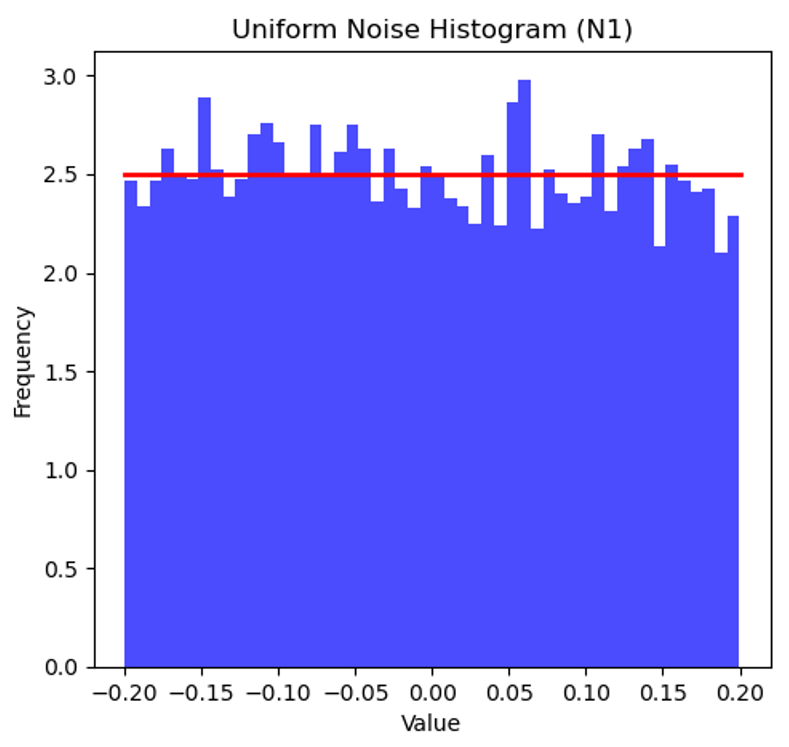
\includegraphics[width=\textwidth]{figures/uniform_noise_dist.PNG}
			\caption{Uniform}
		\end{subfigure}
		\hspace{0.5cm}
		\begin{subfigure}[b]{0.45\textwidth}
			\centering
			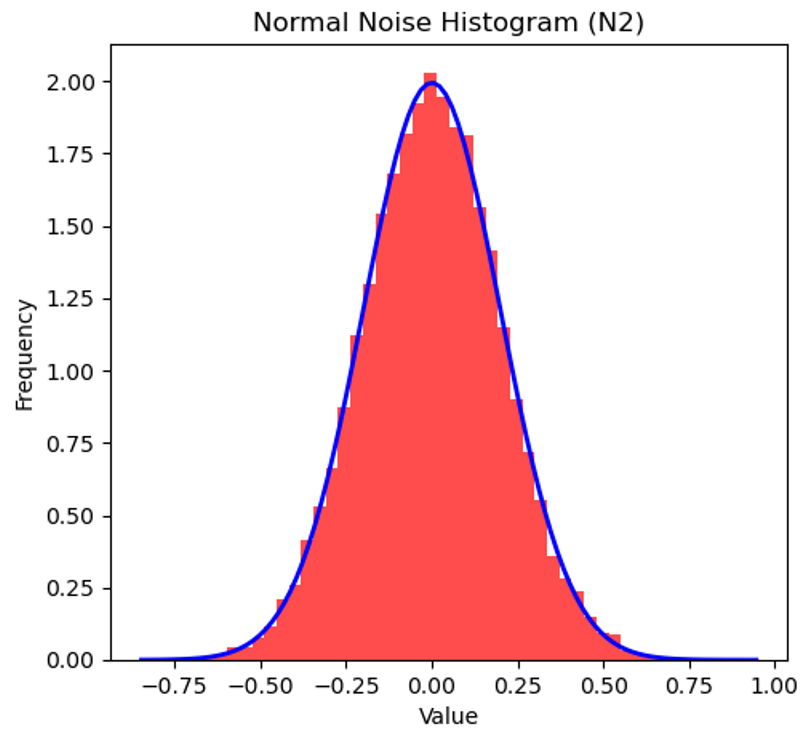
\includegraphics[width=\textwidth]{figures/normal_noise_dist.PNG}
			\caption{Normal}
		\end{subfigure}
		\caption{Histogram plot of noise}
	\end{figure}
	
	\pagebreak
	
	\subsubsection*{(b) Mean of Noise Vectors}
	For the noise vector $N_1$, define:
	\[ N_1 = \frac{1}{L} \sum_{i=1}^L N_1[i]. \tag{5} \]
	
	 Compute $N_1$ for $L \in \{1, 2, \dots, 1000\}$ and plot it as a function of $L$. Repeat the same for $N_2$. What is the limit of $N_1$ and $N_2$ as $L \to \infty$? Which theorem or statement in probability theory precisely explains this result?
	\\ \\
	First we plot the mean for each one as the number of samples increases.
	\begin{figure}[h!]
		\centering
		\begin{subfigure}[b]{0.45\textwidth}
			\centering
			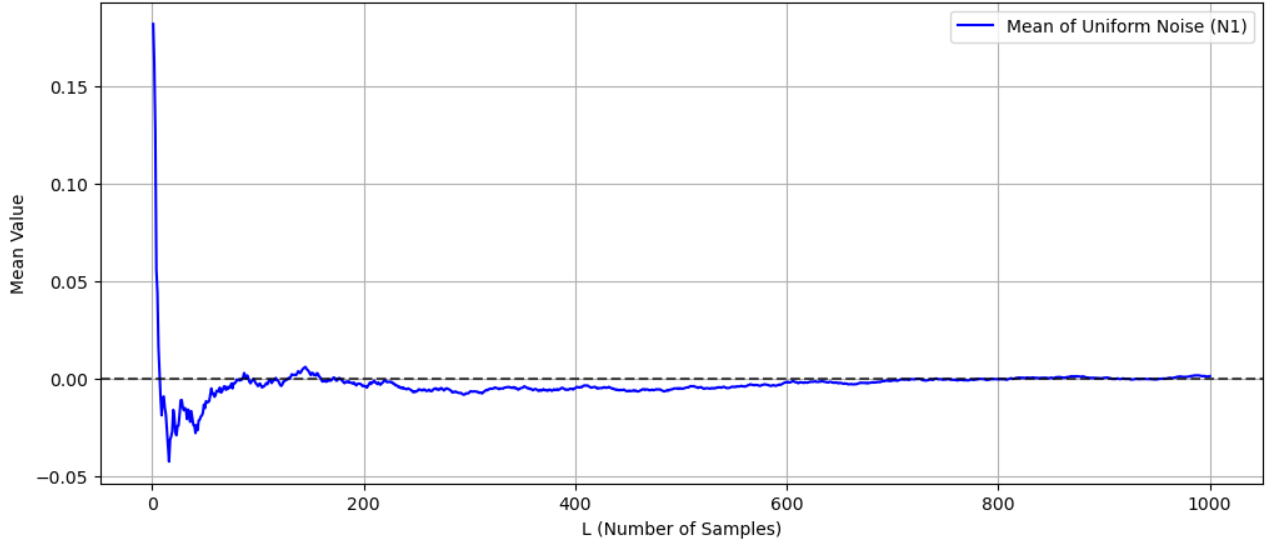
\includegraphics[width=\textwidth]{figures/mean_uniform_dist.PNG}
			\caption{Uniform}
		\end{subfigure}
		\hspace{0.5cm}
		\begin{subfigure}[b]{0.45\textwidth}
			\centering
			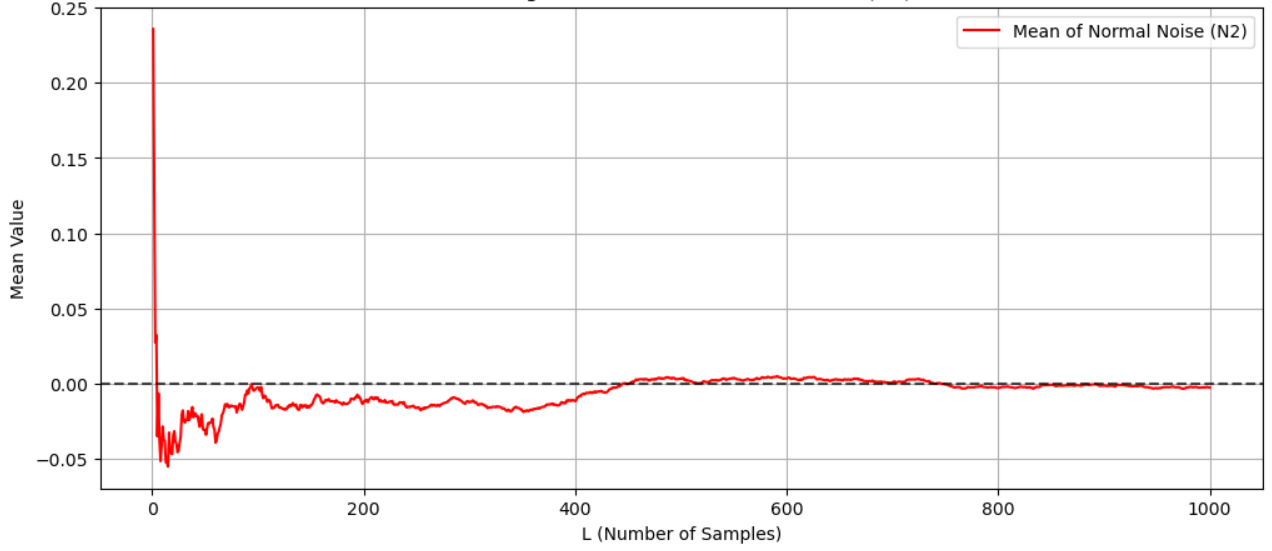
\includegraphics[width=\textwidth]{figures/mean_normal_dist.PNG}
			\caption{Normal}
		\end{subfigure}
		\caption{Convergence of Mean}
	\end{figure}
	
	 As we can as N grows larger, the mean converges. We can justify our results by the Law of Large Numbers (LLN). LLN states that the average of the results obtained from a large number of independent random samples converges to the true value. Since in both of our distributions the mean is 0, both of them converge to 0.
	
	
	
	\subsubsection*{(c) Energy of Noise Vectors}
	Consider the following definition of the energy of a noise vector $N$:
	\[ E_N = \frac{1}{L} \sum_{i=1}^L \left(N[i]\right)^2. \tag{6} \]
	
	 For each of the two noise vectors $N_1$ and $N_2$, compute the energy as a function of $L$ for $L \in \{1, 2, \dots, 1000\}$, and plot it. What is the limit of $E_{N_1}$ and $E_{N_2}$ as $L \to \infty$? Verify your result through simulation.
	\\ \\
	First we calculate the theoretical energy of our signals. Since the mean is 0 for both of them, $E_N = \sigma^2$.
	\\
	$$
	E_N \, [\mathcal{N}(0,a^2)] = a^2
	$$
	$$
	E_N \, [U(-a,a)] = \frac{(a-(-a))^2}{12} = \frac{a^2}{3}
	$$
	
	\pagebreak
	
	\begin{figure}[h!]
		\centering
		\begin{subfigure}[b]{0.45\textwidth}
			\centering
			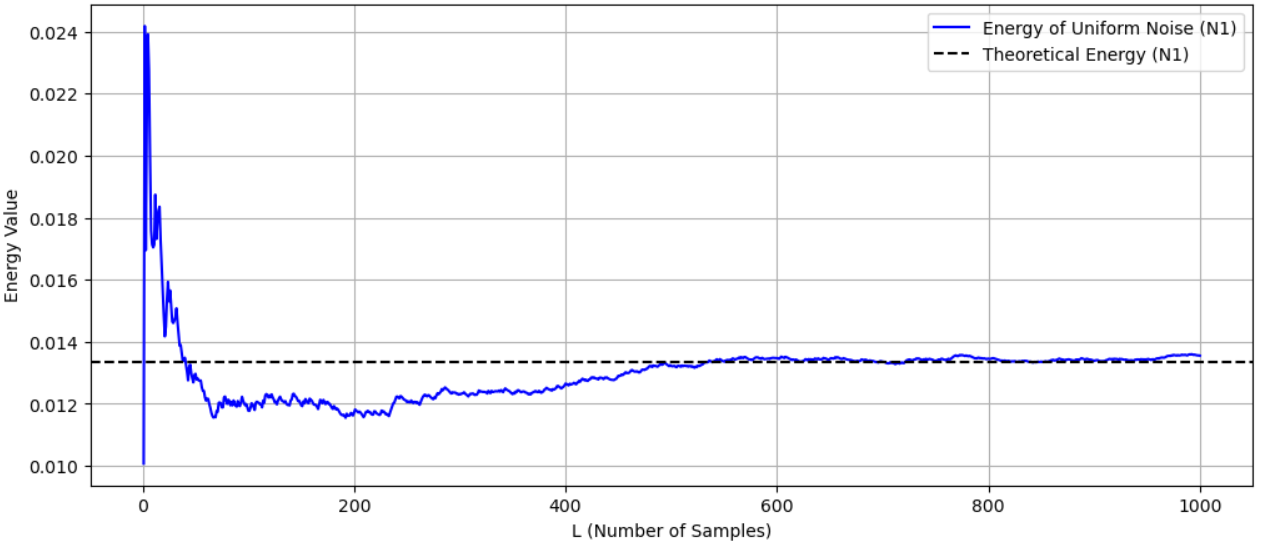
\includegraphics[width=\textwidth]{figures/uniform_energy.PNG}
			\caption{Uniform}
		\end{subfigure}
		\hspace{0.5cm}
		\begin{subfigure}[b]{0.45\textwidth}
			\centering
			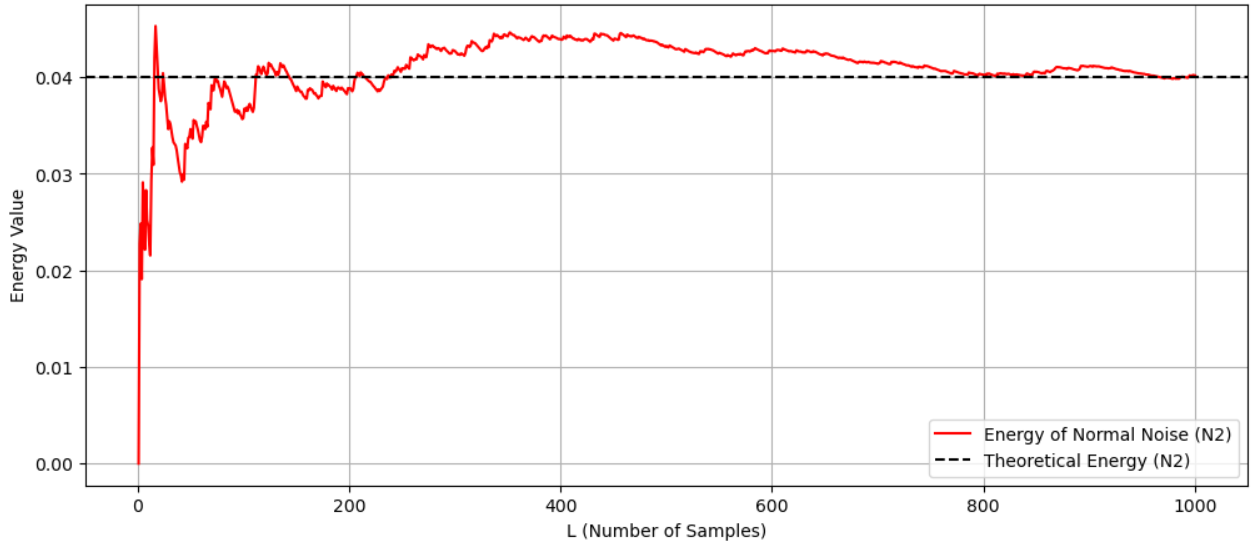
\includegraphics[width=\textwidth]{figures/normal_energy.PNG}
			\caption{Normal}
		\end{subfigure}
		\caption{Convergence of Energy}
	\end{figure}
	
	As we can see from the figures above, as L increases, $E_N$ converges to its theoretical value.
	
	
	\subsubsection*{(d) Cross-Correlation of Noise Vectors}
	For the two noise vectors $N_1$ and $N_2$, define:
	\[ c_{12} = \frac{1}{L} \sum_{i=1}^L N_1[i] N_2[i]. \tag{7} \]
	
	 Plot $c_{12}$ as a function of $L$ for $L \in \{1, 2, \dots, 1000\}$. Also, compute the limit of $c_{12}$ as $L \to \infty$ and verify it through simulation. Explain what information $c_{12}$ provides about the two vectors. Justify how $c_{12}$ serves as a measure of similarity.
	\\ \\
	First we calculate their Cross-Correlation, using probability theory.
	\begin{equation*}
		\begin{split}
			\left.
			\begin{alignedat}{4}
				Cov(N_1, N_2) = E[N_1 N_2] - E[N_1] E[N_2]\\
				E[N_1] = E[N_2] = 0 \\
				\text{both are independent}
			\end{alignedat}
			\right \}
			\Rightarrow Cov(N_1, N_2) = 0
		\end{split}
	\end{equation*}
	
	 Since the expected value of both distributions is zero, $c_{12}$ is equal to the $Cov(N_1, N_2)$. And as we know covariance indicates how the values of two random variables move relative to each other.
	
	\begin{figure}[h!]
		\centering
		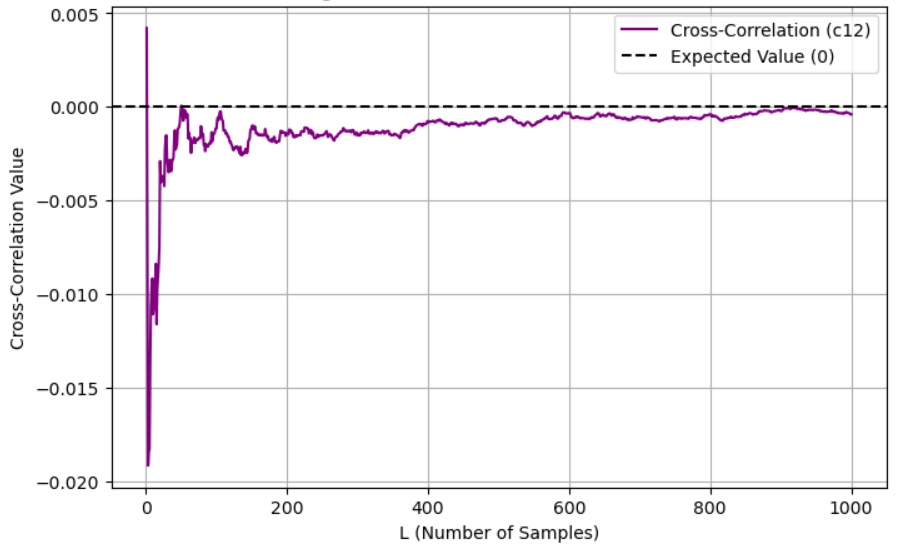
\includegraphics[scale=0.5]{figures/cross_correlation.png}
		\caption{Cross Correlation}
	\end{figure}
	
	\pagebreak
	
	\subsubsection{Sinusoidal Signal and Noise Addition} \label{sec:noise_addition}
	 In this question, the original signal used is a simple sinusoidal signal defined as:
	\[ x(t) = \sin(2\pi f_0 t), \quad f_0 = 1 \text{ Hz}. \]
	
	 The time range of the signal is considered as \([0, 2]\). Generate the signal $x(t)$ with an appropriate sampling frequency. Plot $x(t)$ and specify the sampling frequency used.
	
	 Next, add the noise vectors $N_1$ and $N_2$ to the generated signal to produce two noisy signals $x_{n1}$ and $x_{n2}$:
	\[ x_{n1}(t) = x(t) + N_1(t), \quad x_{n2}(t) = x(t) + N_2(t). \tag{8} \]
	
	 Plot both noisy signals.
	\\ \\
	 We pick 1000 $\frac{\text{samples}}{\text{s}}$ for sampling rate to have a smooth curve.
	
	\begin{figure}[h!]
		\centering
		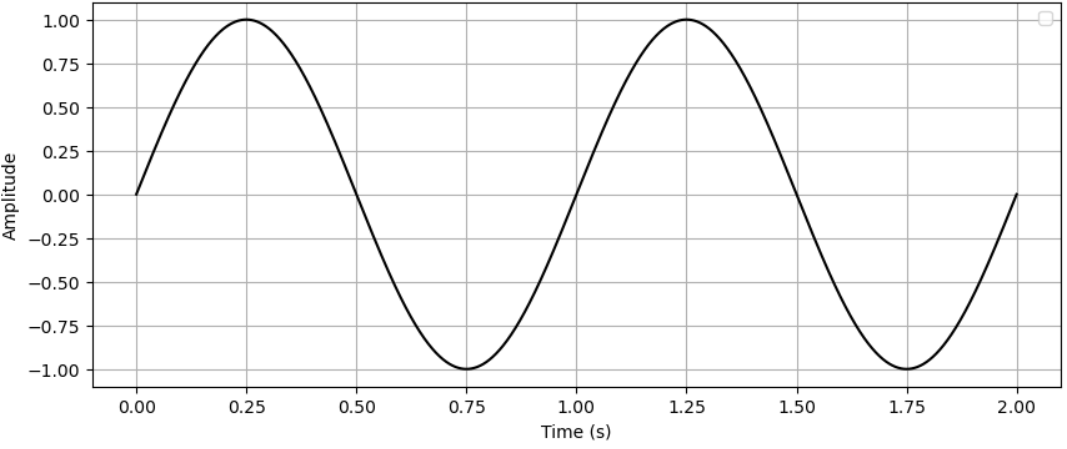
\includegraphics[scale=0.7]{figures/sin.png}
		\caption{Original signal (sine wave)}
	\end{figure}
	
	\begin{figure}[h!]
		\centering
		\begin{subfigure}[b]{0.45\textwidth}
			\centering
			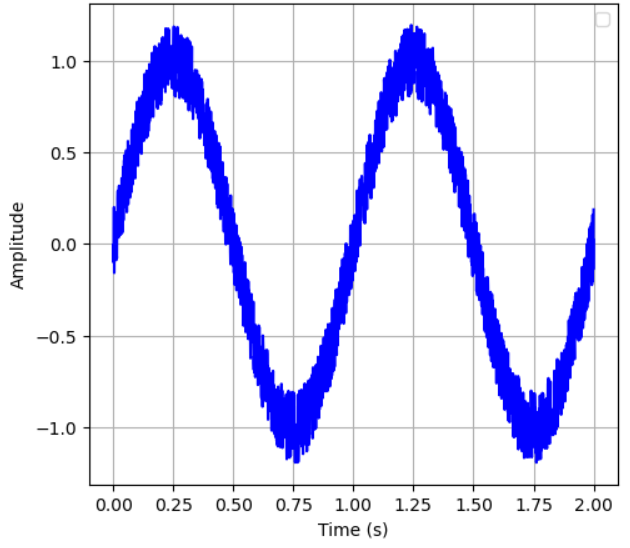
\includegraphics[width=\textwidth]{figures/sin_uniform_noise.PNG}
			\caption{signal with uniform noise}
		\end{subfigure}
		\hspace{0.5cm}
		\begin{subfigure}[b]{0.45\textwidth}
			\centering
			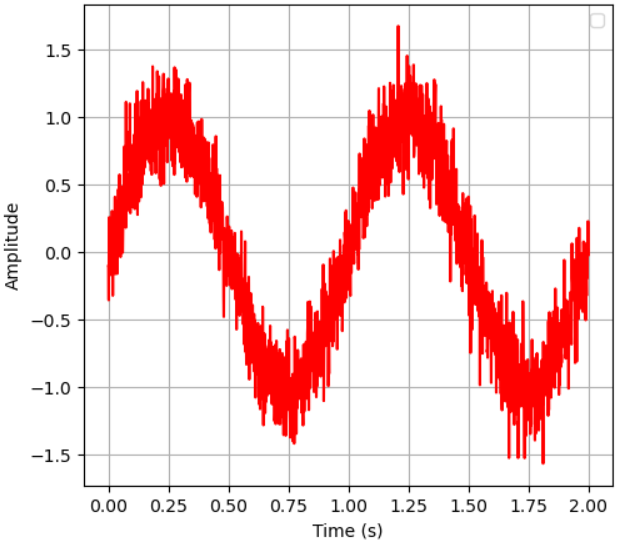
\includegraphics[width=\textwidth]{figures/sin_normal_noise.PNG}
			\caption{signal with normal noise}
		\end{subfigure}
		\caption{Noisy signals}
	\end{figure}
	
	
	\subsubsection{Energy Computation of Signals}
	Compute the energy of the following signals:
	\begin{itemize}
		\item The original signal $x$.
		\item The noise vectors $N_1$ and $N_2$.
		\item The noisy signals $x_{n1}$ and $x_{n2}$.
	\end{itemize}
	
	 In total, compute the energies of five signals. Report the computed energy values. Verify whether the relation $E_{x_n} = E_x + E_N$ approximately holds. For any two signals $x$ and $y$, determine if the statement $E_{x+y} = E_x + E_y$ is true or false. Prove or disprove the statement and validate it for this specific example.
	
	 The calculated values are as follows.
	
	\begin{table}[h!]
		\centering
		\begin{tabular}{c|c|c|c|c|c|}
			\cline{2-6}
			& $E_x$  & $E_{noise}$ & $E_{x} + E_{noise}$ & $E_{xn}$ & Relative Difference \\ \hline
			\multicolumn{1}{|c|}{Uniform Noise (N1)} & 0.4998 & 0.0134      & 0.5132              & 0.5236      & $\sim$2\%           \\ \hline
			\multicolumn{1}{|c|}{Normal Noise (N2)}  & 0.4998 & 0.0392      & 0.539               & 0.5350      & $\sim$0.7\%         \\ \hline
		\end{tabular}
		\caption{}
	\end{table}
	
	
	 Since the differences are relatively small we can say that $E_{x_n} = E_x + E_N$ holds. The discrepancy can be justified by the fact that our sampling size is finite, so if we increasing our sample size, the difference between the theoretical value and the experimental value will shrink.
	\\
	
	 \textbf{Energy Additivity for Any Two Signals}
	Given a discrete signal $x$, its energy is defined as:
	$$
	E_x = \sum_{i} x_i^2
	$$
	For two signals $x$ and $y$, their sum $x + y$ has energy:
	$$
	E_{x+y} = \sum_{i} (x_i + y_i)^2 = \sum_{i} x_i^2 + \sum_{i} y_i^2 + 2\sum_{i} x_i y_i
	$$
	which simplifies to:
	$$
	E_{x+y} = E_x + E_y + 2 \sum_{i} x_i y_i
	$$
	Conclusion: The equation $E_{x+y} = E_x + E_y$ holds only if $\sum_{i} x_i y_i = 0$, meaning $x$ and $y$ must be \textbf{orthogonal} (uncorrelated). In general, the equation is \textbf{false} due to the third term. In our case, since the sine wave and the noise are uncorrelated, this equation holds.
	
	\pagebreak
	
	\subsubsection{Signal-to-Noise Ratio (SNR)}
	The ratio of the energy (power) of the original signal to the energy (or power) of the noise is called the Signal-to-Noise Ratio (SNR):
	\[ \text{SNR} = \frac{E_x}{E_N}. \]
	
	 Compute and report the SNR for the signals $x_{n1}$ and $x_{n2}$ generated in Section~\ref{sec:noise_addition}.
	
	 Subsequently, increase the value of $a$ in the noise definitions until the smallest value of $a$ is found such that there is no noticeable visual similarity between $x$ and $x_n$. Report the corresponding value of $a$ and the SNR for each type of noise separately.
	\\ \\
	We have calculated $E_x$ and $E_N$ of two signals in the previous section. We have:
	$$
	SNR_1 (\text{Uniform}) = \frac{0.49975}{0.01344} \approx 37.2
	$$
	$$
	SNR_2 (\text{Normal}) \approx \frac{0.4998}{0.0392} \approx 12.7
	$$
	
	 We plot our noisy signals for different values of noise amplitude (a). The following images approximately show the transition from recongnizability to unrecognizablity.
	
	\begin{figure}[!h]
		\centering
		\begin{tabular}{c}
			\begin{subfigure}[h]{0.3\textwidth}
				\centering
				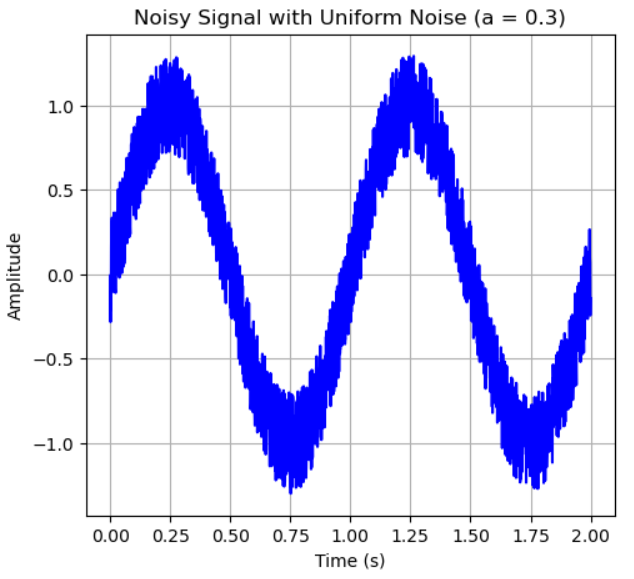
\includegraphics[width=\textwidth]{figures/uniform_noise/0.3.png}
			\end{subfigure}
			\hfill
			\begin{subfigure}[h]{0.3\textwidth}
				\centering
				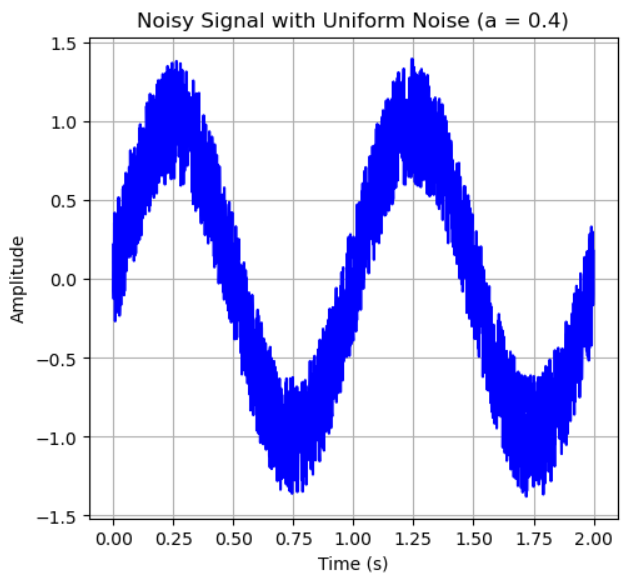
\includegraphics[width=\textwidth]{figures/uniform_noise/0.4.png}
			\end{subfigure}
			\hfill
			\begin{subfigure}[h]{0.3\textwidth}
				\centering
				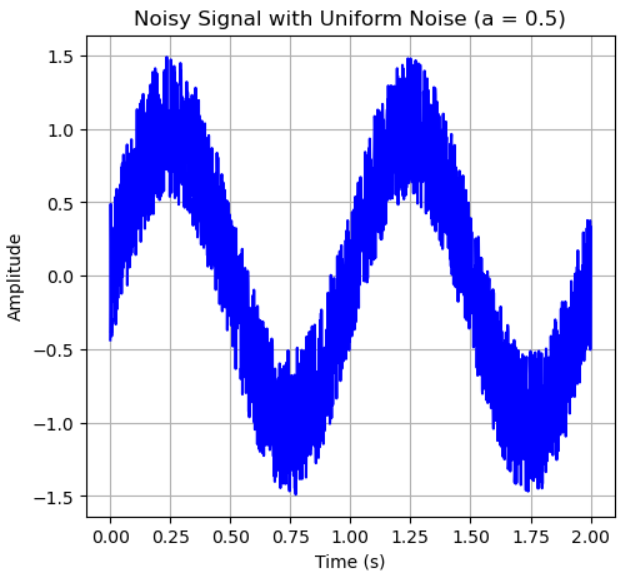
\includegraphics[width=\textwidth]{figures/uniform_noise/0.5.png}
			\end{subfigure} \\
			
			\begin{subfigure}[h]{0.3\textwidth}
				\centering
				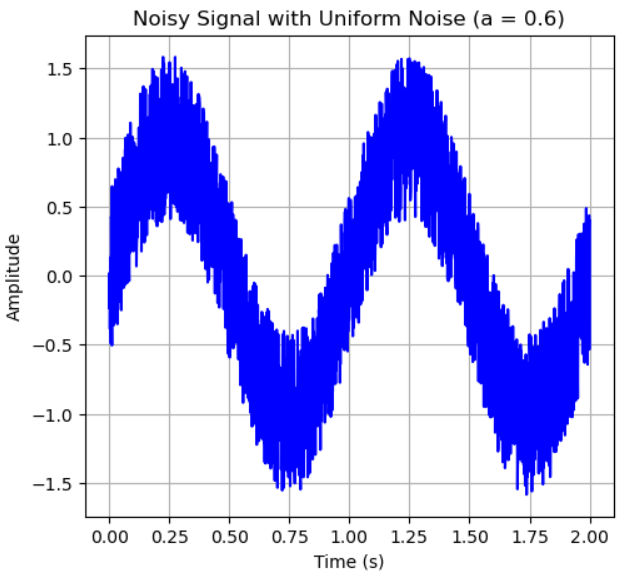
\includegraphics[width=\textwidth]{figures/uniform_noise/0.6.png}
			\end{subfigure}
			\hfill
			\begin{subfigure}[h]{0.3\textwidth}
				\centering
				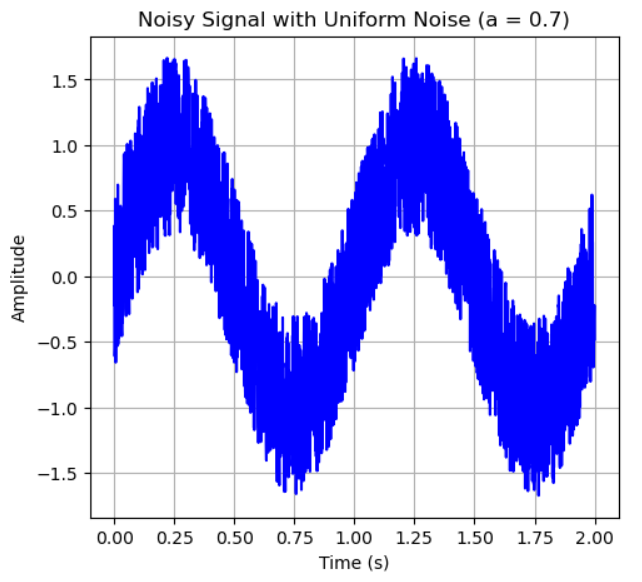
\includegraphics[width=\textwidth]{figures/uniform_noise/0.7.png}
			\end{subfigure}
			\hfill
			\begin{subfigure}[h]{0.3\textwidth}
				\centering
				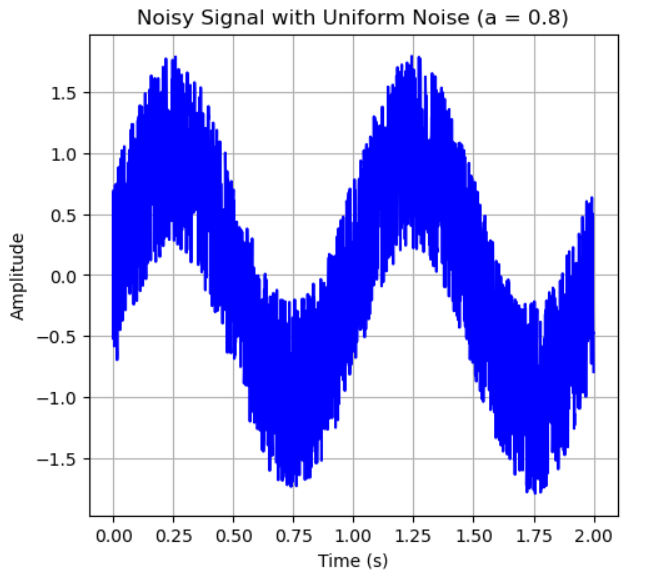
\includegraphics[width=\textwidth]{figures/uniform_noise/0.8.png}
			\end{subfigure} \\
			
		\end{tabular}
		\caption{Uniform noise with different Amplitudes}
	\end{figure}
	
	 We can see that around $a=0.5,\,0.6$, our signal doesn't not visually resemble a sine wave anymore. For instance, the original signal could have been a triangular wave.
	
	\pagebreak
	
	
	\begin{figure}[!h]
		\centering
		\begin{tabular}{c}
			\begin{subfigure}[h]{0.3\textwidth}
				\centering
				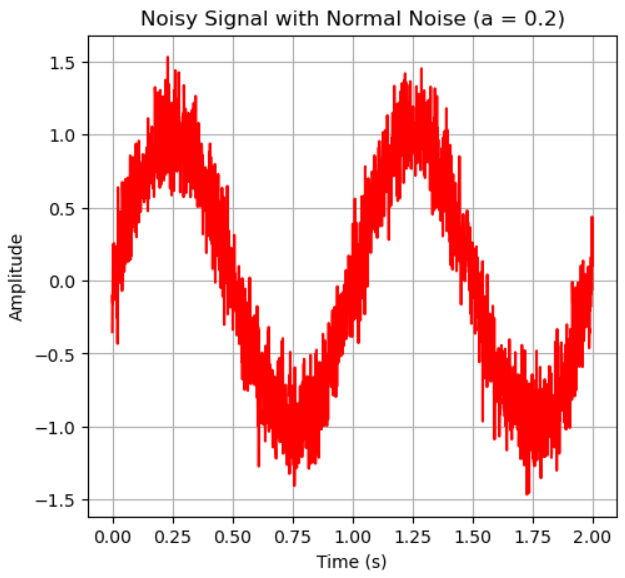
\includegraphics[width=\textwidth]{figures/normal_noise/0.2.png}
			\end{subfigure}
			\hfill
			\begin{subfigure}[h]{0.3\textwidth}
				\centering
				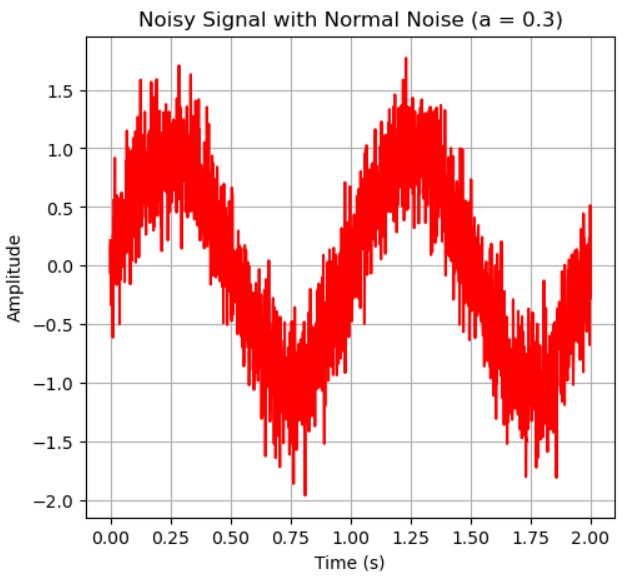
\includegraphics[width=\textwidth]{figures/normal_noise/0.3.png}
			\end{subfigure}
			\hfill
			\begin{subfigure}[h]{0.3\textwidth}
				\centering
				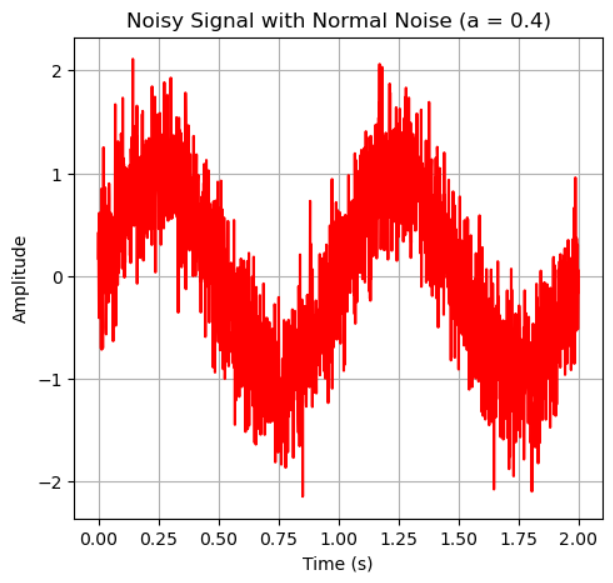
\includegraphics[width=\textwidth]{figures/normal_noise/0.4.png}
			\end{subfigure} \\
			
			\begin{subfigure}[h]{0.3\textwidth}
				\centering
				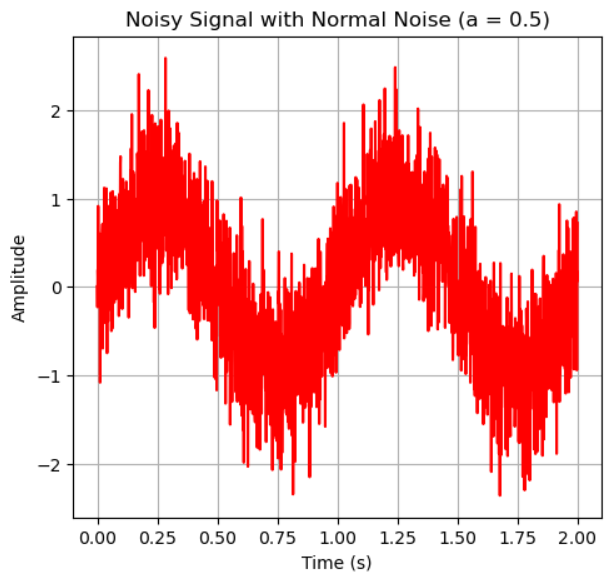
\includegraphics[width=\textwidth]{figures/normal_noise/0.5.png}
			\end{subfigure}
			\hfill
			\begin{subfigure}[h]{0.3\textwidth}
				\centering
				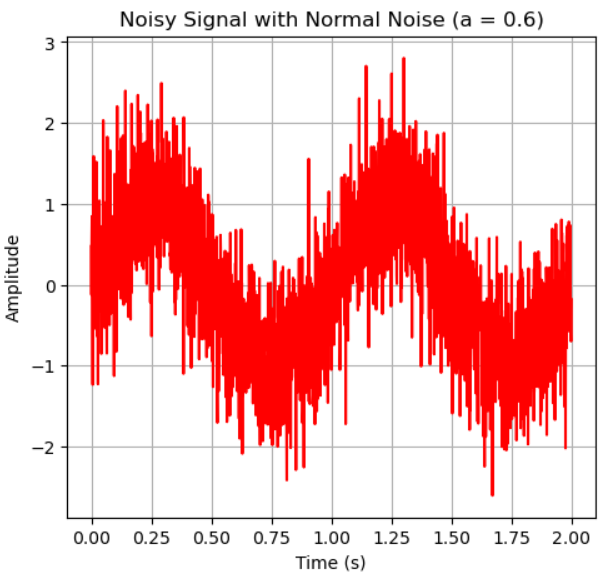
\includegraphics[width=\textwidth]{figures/normal_noise/0.6.png}
			\end{subfigure}
			\hfill
			\begin{subfigure}[h]{0.3\textwidth}
				\centering
				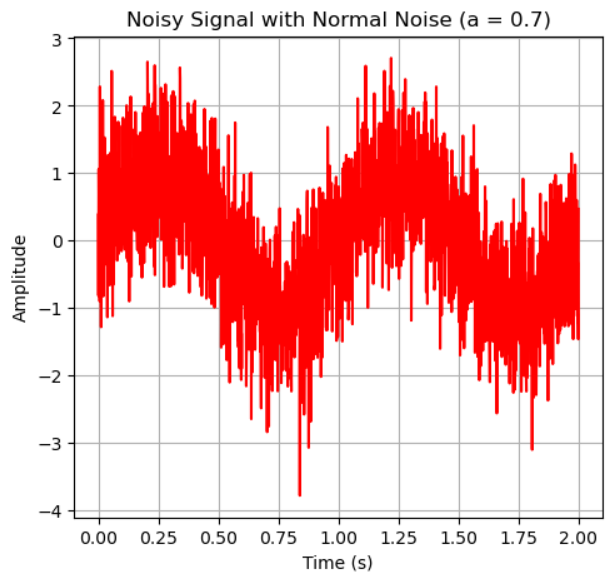
\includegraphics[width=\textwidth]{figures/normal_noise/0.7.png}
			\end{subfigure} \\
			
		\end{tabular}
		\caption{Normal noise with different Amplitudes}
	\end{figure}
	
	
	 We can see that around $a=0.3,\,0.4$, our signal doesn't not visually resemble a sine wave anymore.
	\\ \\
	 It is not strange that the amplitude threshold is lower for normal noise. Since normal distribution is unbounded, even for small values of $a$, large deviations could occur.
	
	\pagebreak
	
	
	\section{Magnetic Resonance Imaging (MRI): A Comprehensive Overview}
	\subsection{Introduction}
	
	Magnetic Resonance Imaging (MRI) is a non-invasive diagnostic technique that produces detailed images of the internal structures of the body. Utilizing strong magnetic fields and radio waves, MRI scans help in diagnosing a variety of conditions by revealing differences between healthy and diseased tissue.
	
	\subsection{How MRI works}
	
	MRI operates on the principles of nuclear magnetic resonance. Here's a step-by-step explanation:
	
	\begin{itemize}
		\item \textbf{Magnetic Alignment}: The human body is composed largely of water molecules, which contain hydrogen nuclei (protons). When a person enters the MRI scanner, a powerful magnetic field aligns these protons.
		\item \textbf{Radiofrequency Pulses}: Short bursts of radio waves are directed at the aligned protons, knocking them out of their equilibrium state.
		\item \textbf{Signal Emission}: When the radiofrequency pulse is turned off, the protons realign with the magnetic field, releasing energy in the process.
		\item \textbf{Image Formation}: This released energy is detected by coils in the scanner. Computers process these signals to construct detailed images of the body's interior.
	\end{itemize}
	
	
	\subsection{Brain MRI}
	MRI is particularly valuable for neurological applications due to its superior contrast resolution, which allows for:
	\begin{itemize}
		\item \textbf{Detection of Tumors and Lesions} : Identifying brain tumors, cysts, and other anomalies.
		\item \textbf{Stroke Evaluation}: Differentiating between ischemic and hemorrhagic strokes.
		\item \textbf{Multiple Sclerosis (MS)}: Visualizing demyelinating plaques characteristic of MS.
		\item \textbf{Aneurysm and Vascular Malformations}: Assessing blood vessel integrity and abnormalities.
		\item \textbf{Infection and Inflammation}: Detecting conditions like encephalitis or abscesses.
	\end{itemize}
	
	\pagebreak
	
	\subsection{Spine MRI}
	Spine MRI provides critical information about spinal anatomy and pathology:
	\begin{itemize}
		\item \textbf{Disc Disorders}: Diagnosing herniated or degenerated discs.
		\item \textbf{Spinal Cord Compression}: Identifying causes of spinal cord pressure, such as tumors or bone fragments.
		\item \textbf{Inflammation and Infections}: Detecting osteomyelitis or epidural abscesses.
		\item \textbf{Congenital Anomalies}: Assessing birth defects affecting the spine.
		\item \textbf{Trauma}: Evaluating injuries to vertebrae, discs, ligaments, and the spinal cord itself.
	\end{itemize}
	
	\subsection{Questions}
	
	Explore the main sources of noise in this method and suggest some ways to deal with these problems.
	
	\vspace{2cm}
	
	\begin{figure}[h!]
		\centering
		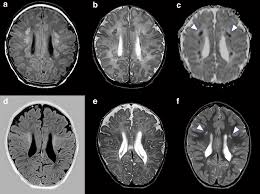
\includegraphics[width=0.7\textwidth]{figures/pic4.jpeg} 
		\caption{Brain MRI}
	\end{figure}
	
	\pagebreak
	
	
	
	\subsubsection{Causes of Noise in Brain and Spine MRI}
	
	The causes of noise in both cases are very similar. Though it is worth separating them to see their difference as well.
	
	 \textbf{Brain MRI:}
	The following are the primary sources of noise in brain MRI.
	
	\begin{enumerate}
		\item \textbf{Motion Artifacts}: Involuntary head movements, such as breathing or swallowing can cause motion-related artifacts.
		
		\item \textbf{Thermal Noise}: Generated by random electrical fluctuations in the scanner's hardware and the thermal behavior of tissues in the brain.
		
		\item \textbf{Magnetic Field Inhomogeneities}: Happens due to flaws in the main magnetic field, which can get worse if there are nearby metal objects like dental fillings or implants.
		
		\item \textbf{External Electromagnetic Interference (EMI)}: Disruptions from external electronic devices or power sources can degrade image quality.
	\end{enumerate}
	
	 \textbf{Spine MRI}
	The following are the primary sources of noise in spine MRI:
	
	\begin{enumerate}
		\item \textbf{Motion Artifacts}: Patient discomfort while lying flat for extended periods can lead to movement which causes noise.
		
		\item \textbf{Thermal Noise}: Similar to brain MRI, but the elongated anatomy of the spine increases susceptibility to hardware noise accumulation over the scan area.
		
		\item \textbf{Magnetic Field Inhomogeneities}: Spine MRI is more affected due to the complex anatomy, including bones, soft tissues, and air in the thoracic region. Variations in the magnetic field occur along the spine's long axis.
		
		\item \textbf{External Electromagnetic Interference (EMI)}: Similar to brain MRI, but has a relatively lower impact as spine imaging typically focuses on larger anatomical structures.
	\end{enumerate}
	
	
	\subsubsection{Approaches to Reduce Noise in MRI}
	
	\subsubsection*{Practical Methods to Minimize Noise}
	\begin{enumerate}
		\item \textbf{Shielded MRI Rooms}: Equip MRI rooms with Faraday cages and magnetic shielding to reduce electromagnetic interference (EMI) from external devices and power lines.
		
		\item \textbf{Motion Reduction}: Provide clear instructions to patients to stay still during the scan and use restraints or padding to minimize involuntary movements.
		
		\item \textbf{Comfort Enhancements}: Ensure patient comfort (e.g., soft headrests, lumbar support) to reduce discomfort and subsequent motion.
		
	\end{enumerate}
	
	\subsubsection*{Algorithmic Approaches to Noise Reduction}
	
	\begin{enumerate}
		\item \textbf{Spatial Filtering}: This technique involves using filters like Gaussian or median filters to process the image. The Gaussian filter smooths the image by reducing sharp variations, which helps in minimizing random noise without losing too much detail. The median filter works by replacing each pixel's value with the median value of its neighboring pixels, effectively removing noise while preserving edges and important details in the image.
		
		\item \textbf{Bayesian Denoising}: This method improves image quality by using prior knowledge about the characteristics of both the original signal and the noise. It applies statistical models to estimate the most likely version of the clean image, considering how the noise might have affected the original data. This approach is especially useful when the noise pattern is complex and not easily removed by simple filters.
		
		\item \textbf{Image Averaging}: In this method, multiple images or scans of the same area are taken and then combined by averaging their pixel values. Since the actual image content remains consistent across the scans, while random noise varies, averaging helps to cancel out the noise. This results in a clearer and more detailed image, as the consistent features are reinforced, and the random noise is reduced.
	\end{enumerate}
	
	
	
	\pagebreak
	
	
	\section{Filters}
	In this part we learn about different filters, how they work and what’s their impact on image. Then using these filters, we denoise two given noisy images and measure how effective each filter is. We are not allowed to use built-in functions for this part.
	\\ \\
	 In this section, we use the image below as an example.
	\begin{figure}[bh!]
		\centering
		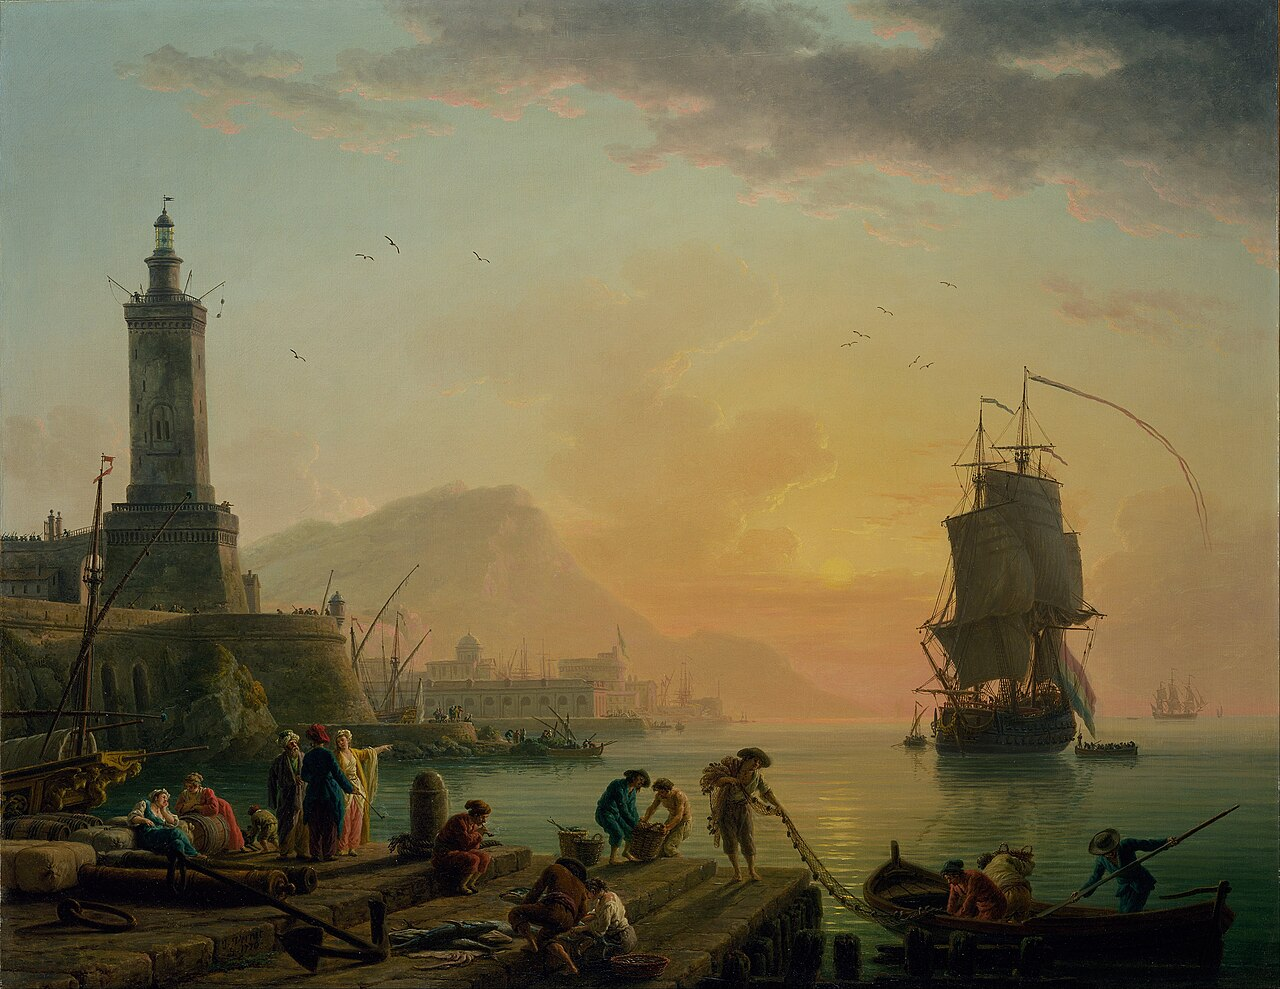
\includegraphics[scale=0.22]{figures/A_Calm_at_a_Mediterranean_Port.jpg}
		\caption{A Calm at a Mediterranean Port | Joseph Vernet}
	\end{figure}
	
	\begin{figure}[bh!]
		\centering
		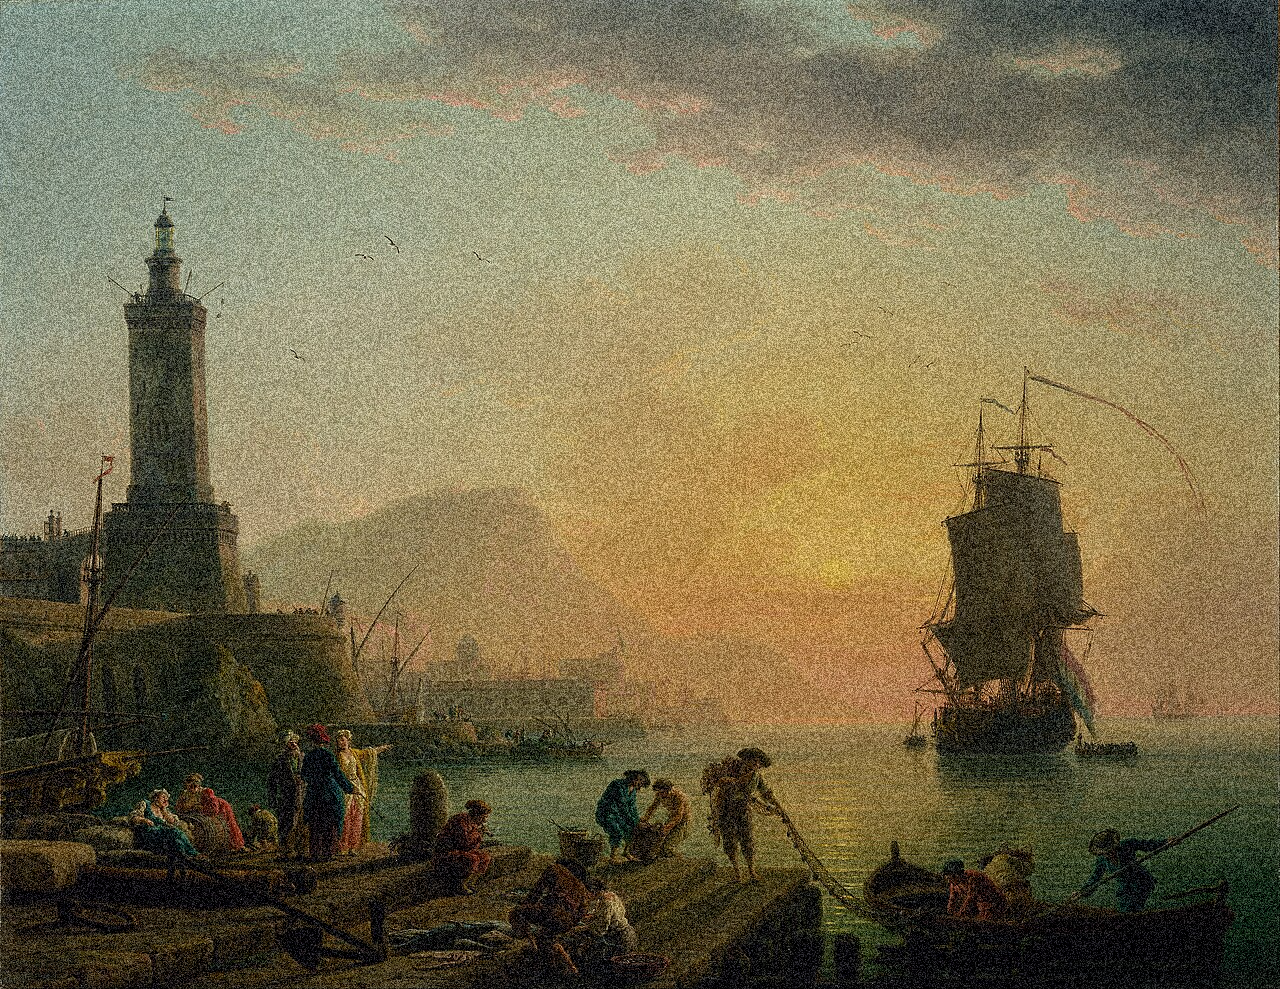
\includegraphics[scale=0.22]{figures/A_Calm_at_a_Mediterranean_Port_noisy.png}
		\caption{Noisy Version of the Image}
		\label{fig:noisy_painting}
	\end{figure}
	
	\pagebreak
	\subsection{Mean Filter}
	The mean filter is a smoothing technique. It works by averaging the pixel values in a local window (kernel) around each pixel, replacing the center pixel with this average. This process blurs the image slightly, making edges and details less sharp while reducing random variations. Larger kernel sizes result in stronger smoothing effects, but they also cause more loss of detail.
	
	\begin{figure}[!h]
		\centering
		\begin{tabular}{c}
			\begin{subfigure}[h]{0.5\textwidth}
				\centering
				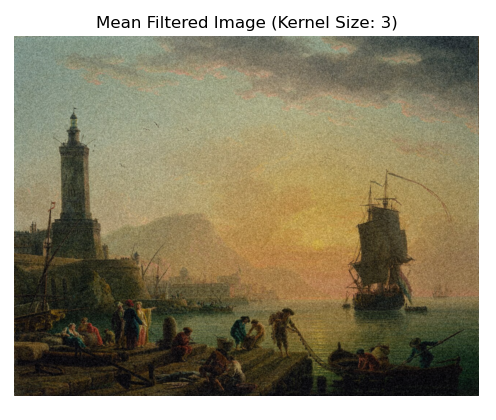
\includegraphics[width=\textwidth]{figures/mean_filter/k_3.png}
			\end{subfigure}
			\hfill
			\begin{subfigure}[h]{0.5\textwidth}
				\centering
				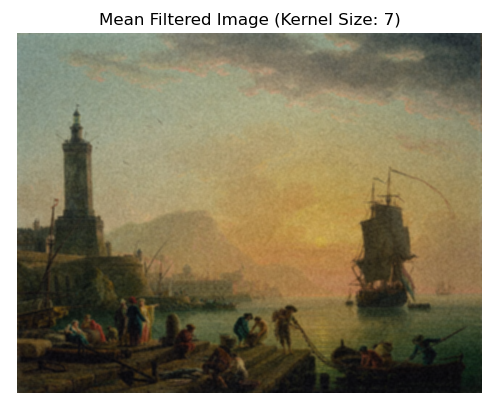
\includegraphics[width=\textwidth]{figures/mean_filter/k_7.png}
			\end{subfigure} \\
			
			\begin{subfigure}[h]{0.5\textwidth}
				\centering
				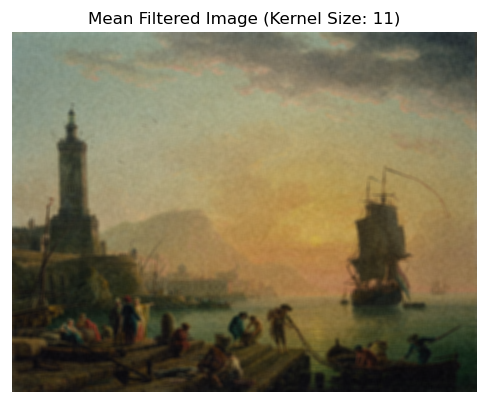
\includegraphics[width=\textwidth]{figures/mean_filter/k_11.png}
			\end{subfigure}
			\hfill
			\begin{subfigure}[h]{0.5\textwidth}
				\centering
				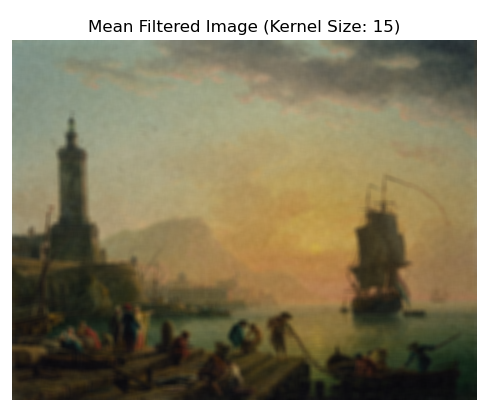
\includegraphics[width=\textwidth]{figures/mean_filter/k_15.png}
			\end{subfigure}
		\end{tabular}
		\caption{Mean Filter with Different Kernel Sizes}
	\end{figure}
	
	\pagebreak
	
	
	\subsection{Gaussian Filter}
	
	The Gaussian filter is a smoothing technique used in image processing to reduce noise and blur images. It works by convolving the image with a Gaussian function, assigning higher weights to nearby pixels and lower weights to farther pixels, resulting in a smooth transition. A 2D Gaussian kernel is defined as:
	$$
	G(x, y) = \frac{1}{2\pi\sigma^2} e^{-\frac{x^2 + y^2}{2\sigma^2}}
	$$
	
	 where:
	\begin{itemize}
		\item \( (x, y) \) are the coordinates of a pixel relative to the center of the kernel.
		\item \( \sigma \) (sigma) is the \textbf{standard deviation}.
		\item The denominator ensures the kernel sums to \textbf{1} for normalization.
	\end{itemize}
	
	\begin{figure}[h!]
		\centering
		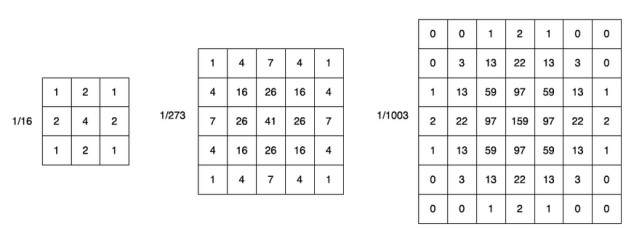
\includegraphics[width=0.9\textwidth]{figures/Gaussian_kernels.jpg} 
		\caption{Discrete approximation of the Gaussian kernels 3x3, 5x5, 7x7}
	\end{figure}
	
	 \textbf{Effects of Kernel Size}
	\begin{itemize}
		\item Determines the \textbf{window size} over which the Gaussian function is applied.
		\item \textbf{Larger kernels} lead to \textbf{more blurring}, as more pixels contribute to the averaging.
	\end{itemize}
	
	 \textbf{Effects of Sigma \( \sigma \)}
	\begin{itemize}
		\item Controls the \textbf{spread} of the Gaussian function.
		\item \textbf{Small sigma} → Sharp details are retained, minor smoothing.
		\item \textbf{Large sigma} → Strong blurring, edges are softened significantly.
	\end{itemize}
	
	\pagebreak
	
	\begin{figure}[!h] 
		\centering
		\resizebox{1.0\textwidth}{!}{
			\begin{tabular}{cccc}
				\begin{subfigure}[h]{0.25\textwidth}
					\centering
					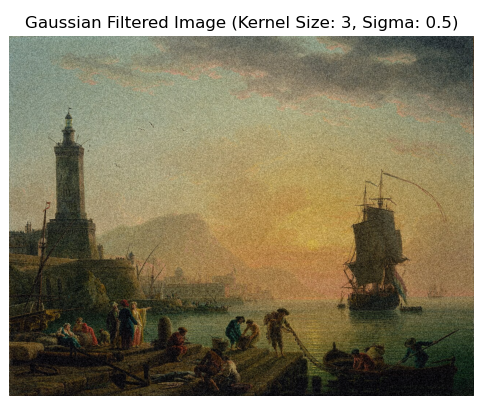
\includegraphics[width=\textwidth]{figures/gaussian_filter/1.png}
				\end{subfigure} &
				\begin{subfigure}[h]{0.25\textwidth}
					\centering
					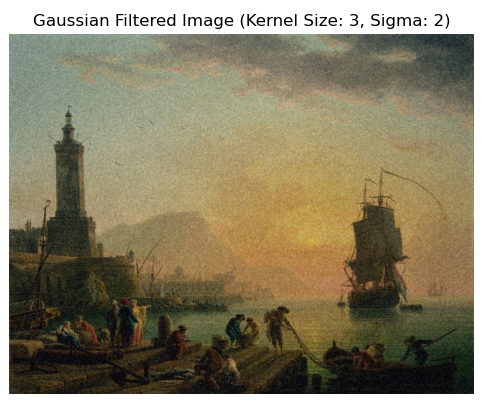
\includegraphics[width=\textwidth]{figures/gaussian_filter/2.png}
				\end{subfigure} &
				\begin{subfigure}[h]{0.25\textwidth}
					\centering
					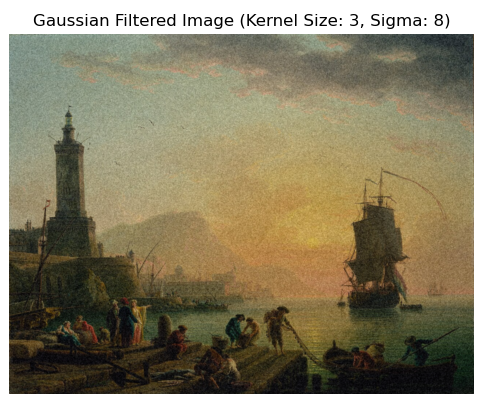
\includegraphics[width=\textwidth]{figures/gaussian_filter/3.png}
				\end{subfigure} &
				\begin{subfigure}[h]{0.25\textwidth}
					\centering
					\includegraphics[width=\textwidth]{figures/gaussian_filter/4.png}
				\end{subfigure} \\
				
				\begin{subfigure}[h]{0.25\textwidth}
					\centering
					\includegraphics[width=\textwidth]{figures/gaussian_filter/5.png}
				\end{subfigure} &
				\begin{subfigure}[h]{0.25\textwidth}
					\centering
					\includegraphics[width=\textwidth]{figures/gaussian_filter/6.png}
				\end{subfigure} &
				\begin{subfigure}[h]{0.25\textwidth}
					\centering
					\includegraphics[width=\textwidth]{figures/gaussian_filter/7.png}
				\end{subfigure} &
				\begin{subfigure}[h]{0.25\textwidth}
					\centering
					\includegraphics[width=\textwidth]{figures/gaussian_filter/8.png}
				\end{subfigure} \\
				
				\begin{subfigure}[h]{0.25\textwidth}
					\centering
					\includegraphics[width=\textwidth]{figures/gaussian_filter/9.png}
				\end{subfigure} &
				\begin{subfigure}[h]{0.25\textwidth}
					\centering
					\includegraphics[width=\textwidth]{figures/gaussian_filter/10.png}
				\end{subfigure} &
				\begin{subfigure}[h]{0.25\textwidth}
					\centering
					\includegraphics[width=\textwidth]{figures/gaussian_filter/11.png}
				\end{subfigure} &
				\begin{subfigure}[h]{0.25\textwidth}
					\centering
					\includegraphics[width=\textwidth]{figures/gaussian_filter/12.png}
				\end{subfigure} \\
				
				\begin{subfigure}[h]{0.25\textwidth}
					\centering
					\includegraphics[width=\textwidth]{figures/gaussian_filter/13.png}
				\end{subfigure} &
				\begin{subfigure}[h]{0.25\textwidth}
					\centering
					\includegraphics[width=\textwidth]{figures/gaussian_filter/14.png}
				\end{subfigure} &
				\begin{subfigure}[h]{0.25\textwidth}
					\centering
					\includegraphics[width=\textwidth]{figures/gaussian_filter/15.png}
				\end{subfigure} &
				\begin{subfigure}[h]{0.25\textwidth}
					\centering
					\includegraphics[width=\textwidth]{figures/gaussian_filter/16.png}
				\end{subfigure}
			\end{tabular}
		}
		\caption{Gaussian Filter with different kernel sizes and sigmas}
	\end{figure}
	
	
	\subsection{Bilateral Filter}
	When we consider how the Gaussian filter works, we notice one problem: it struggles to preserve fine edges. This happens because the filter treats all neighboring pixels based only on their spatial distance from the selected pixel, without considering their brightness. To improve the filter, we can also take the brightness of the pixels into account, which helps in preserving edges while still reducing noise.
	$$
	\text{Gaussian: } I_{\text{filtered}}(x) = \frac{1}{W(x)} \sum_{x_i \in \mathcal{N}(x)} I(x_i) \cdot \exp\left(-\frac{\|x - x_i\|^2}{2\sigma_s^2}\right)
	$$
	
	Now if we add the brightness to our equation, we get:
	$$
	\text{Bilateral: }I_{\text{filtered}}(x) = \frac{1}{W(x)} \sum_{x_i \in \mathcal{N}(x)} I(x_i) \cdot \exp \left( - \frac{\| x - x_i \|^2}{2 \sigma_s^2} \right) \cdot \exp \left(- \frac{\| I(x) - I(x_i) \|^2}{2 \sigma_r^2}\right)
	$$
	
	where:
	\begin{itemize}
		\item \( I(x_i) \) is the intensity of the neighboring pixel at location \( x_i \).
		\item \( \|x - x_i\| \) is the spatial distance between pixel \( x \) and pixel \( x_i \).
		\item \( \sigma_s \) is the spatial standard deviation, controlling how much spatial distance influences the weight.
		\item \( \sigma_r \) is the range standard deviation, controlling how much intensity difference influences the weight.
		\item \( \mathcal{N}(x) \) is the neighborhood of pixel \( x \).
		\item \( W(x) \) is a normalization factor ensuring the sum of the weights is 1.
	\end{itemize}
	This way the value of the current pixel will not be simply calculated based on the spatial distance, now the similarity in brightness plays a role as well. Now we apply this filter to our original image.
	\vspace*{2cm}
	\begin{figure}[h!]
		\centering
		\includegraphics[scale=0.7]{figures/bilateral_filter/1.png}
		\caption{Bilateral Filtered Image (Kernel Size: 5, Sigma Intensity: 25)}
	\end{figure}
	
	\pagebreak
	
	\subsection{Evaluation}
	
	Evaluate the output of the three methods discussed in this section using SNR and PSNR criteria and present the results, compared with the images below in a table. Also, calculate these two criteria for the initial noisy image and declare which method performed better in noise reduction. Can you guess what kind of noise each picture has?
	
		\begin{figure}[!h]
		\centering
			\begin{tabular}{c}
				\begin{subfigure}[h]{0.3\textwidth}
					\centering
					\includegraphics[width=\textwidth]{figures/brain_mri/original.jpg}
					\caption{Original Brain MRI}
				\end{subfigure}
				\hfill
				\begin{subfigure}[h]{0.3\textwidth}
					\centering
					\includegraphics[width=\textwidth]{figures/spine_mri/original.jpg}
					\caption{Original Spine MRI}
				\end{subfigure}
			\end{tabular}
		\caption{}
	\end{figure}
	
	\begin{figure}[!h]
		\centering
		\begin{tabular}{c}
			\begin{subfigure}[h]{0.3\textwidth}
				\centering
				\includegraphics[width=\textwidth]{figures/brain_mri/noisy.jpg}
				\caption{Noisy Brain MRI}
			\end{subfigure}
			\hfill
			\begin{subfigure}[h]{0.3\textwidth}
				\centering
				\includegraphics[width=\textwidth]{figures/spine_mri/noisy.jpg}
				\caption{Noisy Spine MRI}
			\end{subfigure}
		\end{tabular}
		\caption{}
	\end{figure}
	
	\pagebreak
	
	 First we apply each filter and see the results.
	
	\begin{figure}[!h]
		\centering
		\begin{tabular}{c}
			\begin{subfigure}[h]{0.3\textwidth}
				\centering
				\includegraphics[width=\textwidth]{figures/brain_mri/mean.jpg}
				\caption{Mean Filter}
			\end{subfigure}
			\hfill
			\begin{subfigure}[h]{0.3\textwidth}
				\centering
				\includegraphics[width=\textwidth]{figures/brain_mri/gaussian.jpg}
				\caption{Gaussian Filter}
			\end{subfigure}
			\hfill
			\begin{subfigure}[h]{0.3\textwidth}
				\centering
				\includegraphics[width=\textwidth]{figures/brain_mri/bilateral.jpg}
				\caption{Bilateral Filter}
			\end{subfigure}
		\end{tabular}
		\caption{Denoised Brain MRI}
	\end{figure}
	
	\begin{figure}[!h]
		\centering
		\begin{tabular}{c}
			\begin{subfigure}[h]{0.3\textwidth}
				\centering
				\includegraphics[width=\textwidth]{figures/spine_mri/mean.jpg}
				\caption{Mean Filter}
			\end{subfigure}
			\hfill
			\begin{subfigure}[h]{0.3\textwidth}
				\centering
				\includegraphics[width=\textwidth]{figures/spine_mri/gaussian.jpg}
				\caption{Gaussian Filter}
			\end{subfigure}
			\hfill
			\begin{subfigure}[h]{0.3\textwidth}
				\centering
				\includegraphics[width=\textwidth]{figures/spine_mri/bilateral.jpg}
				\caption{Bilateral Filter}
			\end{subfigure}
		\end{tabular}
		\caption{Denoised Spine MRI}
	\end{figure}
	
	Then we calculate the SNR and PSNR by comparing our denoised images with the original one.
	
	\begin{table}[h!]
		\centering
		\begin{tabular}{|c|c|c|}
			\hline
			\textbf{Filter}       & \textbf{PSNR (dB)} & \textbf{SNR (dB)} \\
			\hline
			Mean Filter           & 21.79              & 9.98              \\
			Gaussian Filter       & 22.11              & 10.32             \\
			Bilateral Filter      & 20.37              & 8.32              \\
			\hline
		\end{tabular}
		\caption{Brain MRI Results}
	\end{table}
	
	\begin{table}[h!]
		\centering
		\begin{tabular}{|c|c|c|}
			\hline
			\textbf{Filter}       & \textbf{PSNR (dB)} & \textbf{SNR (dB)} \\
			\hline
			Mean Filter           & 16.53              & 5.64              \\
			Gaussian Filter       & 16.30              & 5.29              \\
			Bilateral Filter      & 17.62              & 7.64              \\
			\hline
		\end{tabular}
		\caption{Spine MRI Results}
	\end{table}
	
	\pagebreak
	
	 Based on the values in the tables:
	
		\textbf{Brain MRI:}
		\begin{itemize}
			\item The Bilateral Filter does not perform as well as the Mean and Gaussian Filters for denoising.
			\item The Mean and Gaussian Filters are known for their effectiveness in smoothing global noise patterns due to their averaging nature, making them suitable for periodic noise.
			\item Therefore, we can infer that the noise in the brain MRI image is likely \textbf{periodic noise}.
		\end{itemize}
		
		\textbf{Spine MRI:}
		\begin{itemize}
			\item The Mean Filter achieves the best results among the three filters.
			\item The Mean Filter is particularly effective at reducing \textbf{salt-and-pepper noise} because it averages pixel intensities within a window, mitigating the impact of extreme outliers caused by scattered white and black dots.
			\item Thus, we can conclude that the noise in the spine MRI image is likely \textbf{salt-and-pepper noise}.
		\end{itemize}
	
	\pagebreak
	
	\section{Adaptive Filter}
	
	\subsection{Questions}
	1. What are finite impulse response (FIR) Adaptive Filters, and What are their specific applications in Biomedical Image Processing? Explore about Wiener filters.
	
	
	\section*{Finite Impulse Response (FIR) Adaptive Filters}
	Finite Impulse Response (FIR) adaptive filters are digital filters that adapt their coefficients based on a specified performance criterion, such as minimizing the mean square error (MSE). These filters rely on a finite number of past input samples to compute their output. Adaptive filters are commonly implemented using algorithms like the Least Mean Squares (LMS) or Recursive Least Squares (RLS), which iteratively update the filter coefficients.
	
	\subsection*{Key Characteristics:}
	\begin{itemize}
		\item \textbf{Finite Impulse Response:} The output depends only on a finite number of input samples, ensuring stability.
		\item \textbf{Adaptability:} The coefficients adjust dynamically to track variations in the input signal or environment.
		\item \textbf{Convergence:} These filters aim to minimize a predefined error function, such as the difference between the filter output and the desired signal.
	\end{itemize}
	
	\subsection*{Applications in Biomedical Image Processing:}
	FIR adaptive filters are widely used in biomedical signal and image processing due to their ability to remove noise, enhance features, and adapt to varying conditions. Specific applications include:
	\begin{enumerate}
		\item \textbf{Noise Reduction:}
		\begin{itemize}
			\item Removes high-frequency noise from MRI, CT, or ultrasound images.
			\item Effective for eliminating noise in biomedical signals (e.g., ECG or EEG) without distorting the underlying signal.
		\end{itemize}
		\item \textbf{Artifact Removal:}
		\begin{itemize}
			\item Removes motion artifacts in dynamic imaging modalities like real-time MRI or X-ray imaging.
			\item Suppresses imaging artifacts caused by patient movement or hardware malfunction.
		\end{itemize}
		\item \textbf{Edge Preservation:} Enhances the edges in medical images while suppressing noise, preserving diagnostically important features.
		\item \textbf{Adaptive Deconvolution:} Enhances resolution in blurred images, such as low-light endoscopic or low-resolution microscopy images.
		\item \textbf{Dynamic Noise Environments:} Particularly useful in imaging systems where noise characteristics change over time, such as real-time imaging or imaging in intensive care units.
	\end{enumerate}
	
	\section*{Wiener Filters}
	Wiener filters are optimal linear filters designed to minimize the mean square error. However, they assume Gaussian noise and may perform sub-optimally for salt-and-pepper noise, as observed in the spine MRI results. between the filtered signal and the desired signal. They rely on a priori knowledge of the signal and noise characteristics, such as their power spectral densities.
	
	\subsection*{Key Characteristics:}
	\begin{itemize}
		\item \textbf{Frequency Domain Approach:} Wiener filters operate in the frequency domain, leveraging information about the signal and noise to suppress unwanted components.
		\item \textbf{Optimality:} These filters provide the best linear estimation of the desired signal under stationary noise and signal conditions.
		\item \textbf{Linear and Non-Adaptive:} Unlike adaptive filters, Wiener filters are fixed and do not adapt in real-time.
	\end{itemize}
	
	\subsection*{Applications in Biomedical Image Processing:}
	\begin{enumerate}
		\item \textbf{Image Denoising:} Commonly used to remove Gaussian noise from medical images, such as CT scans, MRIs, and X-rays.
		\item \textbf{Restoration of Blurred Images:} Restores blurred images by deconvolving the image with the system's point spread function.
		\item \textbf{Enhancement of Medical Signals:} Removes noise from biomedical signals, such as ECG, EEG, or fMRI time series, improving their interpretability.
		\item \textbf{Microscopy Image Restoration:} Corrects for optical blurring in microscopy images, enhancing the visibility of cellular structures.
		\item \textbf{Signal Reconstruction:} Used in image reconstruction tasks, such as reconstructing images from sparse data in CT or MRI.
	\end{enumerate}
	
	\section*{Comparison of FIR Adaptive Filters and Wiener Filters}
	\begin{table}[h!]
		\centering
		\begin{tabular}{|p{3cm}|p{5cm}|p{5cm}|}
			\hline
			\textbf{Feature} & \textbf{FIR Adaptive Filters} & \textbf{Wiener Filters} \\ \hline
			\textbf{Adaptability} & Real-time adaptability to changing noise environments & Non-adaptive, requires prior knowledge of noise characteristics \\ \hline
			\textbf{Application} & Suitable for dynamic and time-varying signals or images & Best for stationary noise and signal conditions \\ \hline
			\textbf{Complexity} & Higher, due to real-time updates of coefficients & Moderate, requires computation of power spectral densities \\ \hline
			\textbf{Key Strength} & Effectively handles non-stationary noise & Optimal performance with stationary noise \\ \hline
			\textbf{Typical Use} & Adaptive noise cancellation, artifact removal & Image restoration, deblurring, and denoising \\ \hline
		\end{tabular}
		\caption{Comparison of FIR Adaptive Filters and Wiener Filters}
	\end{table}
	
	
	
	2. Explore the role of Stochastic Gradient Descent(SGD) in optimizing filter coefficients in real-time, its convergence properties, and its application in adaptive filter design.
	
	\section*{Stochastic Gradient Descent (SGD) in Adaptive Filter Design}
	
	\subsection*{Overview of Stochastic Gradient Descent (SGD)}
	Stochastic Gradient Descent (SGD) is an optimization algorithm used to minimize an objective function, such as the mean square error (MSE). Unlike standard gradient descent, which uses the entire dataset to calculate gradients, SGD updates parameters using only a subset of the data (or a single data point), making it computationally efficient and well-suited for real-time applications.
	
	\subsection*{Role of SGD in Real-Time Filter Optimization}
	In the context of adaptive filters, SGD plays a critical role in optimizing filter coefficients dynamically. Adaptive filters, such as Finite Impulse Response (FIR) filters, adjust their coefficients in real-time to minimize the error between the filter output and the desired signal. SGD enables this real-time adaptation through iterative updates.
	
	\subsubsection*{Key Steps in SGD for Adaptive Filters:}
	\begin{enumerate}
		\item \textbf{Error Computation:} Compute the instantaneous error:
		\[
		e(n) = d(n) - y(n),
		\]
		where \( d(n) \) is the desired signal and \( y(n) \) is the filter output.
		
		\item \textbf{Gradient Estimation:} Estimate the gradient of the error with respect to the filter coefficients.
		
		\item \textbf{Coefficient Update:} Update the filter coefficients \( w_i(n) \) as:
		\[
		w_i(n+1) = w_i(n) + \eta \cdot e(n) \cdot x_i(n),
		\]
		where \( \eta \) is the learning rate and \( x_i(n) \) represents the input signal.
	\end{enumerate}
	
	\subsection*{Convergence Properties of SGD}
	The convergence of SGD is influenced by factors such as the learning rate, input signal characteristics, and the stationarity of the data.
	
	\subsubsection*{Key Factors Affecting Convergence:}
	\begin{itemize}
		\item \textbf{Learning Rate (\( \eta \)):}
		\begin{itemize}
			\item High learning rates lead to faster convergence but may cause instability.
			\item Low learning rates ensure stability but result in slower convergence.
		\end{itemize}
		\item \textbf{Input Signal Characteristics:}
		\begin{itemize}
			\item Stationary signals result in smoother convergence.
			\item Non-stationary signals may introduce oscillations in coefficient updates.
		\end{itemize}
		\item \textbf{Step Size Decay:} Using a decaying learning rate, such as \( \eta = \frac{\eta_0}{1+n} \), improves convergence stability over time.
		\item \textbf{Mean Square Error Surface:} Convergence depends on the curvature of the error surface; flat surfaces require smaller learning rates.
	\end{itemize}
	
	\subsubsection*{Trade-offs:}
	\begin{itemize}
		\item Faster convergence may lead to overshooting or instability.
		\item Slower convergence ensures stability but may not adapt effectively to rapid changes.
	\end{itemize}
	
	\subsection*{Applications in Adaptive Filter Design}
	SGD is widely used in adaptive filter design due to its efficiency and suitability for real-time implementations. Some common applications include:
	
	\begin{enumerate}
		\item \textbf{Noise Cancellation:} Adaptive filters optimized with SGD remove noise from biomedical signals (e.g., ECG, EEG) in real-time.
		\item \textbf{Channel Equalization:} Used in communication systems to mitigate distortion or interference.
		\item \textbf{Echo Cancellation:} Reduces echo effects in telecommunication systems, such as in VoIP and video calls.
		\item \textbf{Time-Varying Environments:} Filters adapt to non-stationary signals, such as dynamic noise in real-time imaging systems.
	\end{enumerate}
	
	\pagebreak
	
	\subsection*{Advantages of SGD in Adaptive Filters:}
	\begin{itemize}
		\item \textbf{Real-Time Adaptation:} Efficient for streaming data with low computational overhead.
		\item \textbf{Scalability:} Handles high-dimensional data, making it suitable for complex filter designs.
		\item \textbf{Simplicity:} Requires minimal storage and computation compared to batch gradient descent.
	\end{itemize}
	
	3. Write a function that applies an Adaptive filter to an input image. Suggest a way to tune learning parameter. Apply this filter to \textcolor{blue}{original\_brain\_MRI.jpg} and \textcolor{blue}{original\_spine\_MRI.jpg}.
	\\ \\
	
	Tuning the learning parameter (or learning rate) is crucial for optimizing algorithms, especially in adaptive filtering techniques like the Least Mean Squares (LMS) approach used for image denoising. The learning rate controls how much the filter’s weights are adjusted at each iteration in response to the error. If the learning rate is too high, the filter may overshoot the optimal solution, leading to instability or poor convergence. Conversely, if the learning rate is too low, convergence can be very slow, potentially leading to suboptimal performance.
	
	One effective method to tune the learning parameter is through error-based iterative optimization. This can be achieved by starting with an initial learning rate and gradually adjusting it to minimize the error (e.g., Mean Squared Error, MSE) between the desired output (reference image) and the filter’s output. A decaying learning rate can be used, where the learning rate is reduced over time as the error decreases, allowing the filter to fine-tune its weights more precisely as it converges. This strategy ensures faster convergence at the beginning and more stable adjustments as the algorithm approaches the optimal solution.
	
	Here are the applied filter to noisy images.
	
	
	\begin{figure}[!h]
		\centering
		\begin{tabular}{c}
			\begin{subfigure}[h]{0.4\textwidth}
				\centering
				\includegraphics[width=\textwidth]{figures/adaptive/brain.jpg}
				\caption{Filtered Brain MRI Image}
			\end{subfigure}
			\hfill
			\begin{subfigure}[h]{0.4\textwidth}
				\centering
				\includegraphics[width=\textwidth]{figures/adaptive/spine.jpg}
				\caption{Filtered Spine MRI Image}
			\end{subfigure}
		\end{tabular}
		\caption{Adaptive Filter}
	\end{figure}
	
	
	\pagebreak
	
	4. Evaluate the output of this method using SNR and PSNR criteria and present the results. Which of these four filters did better for each image? Can you explain why?
	
	
	\begin{table}[h!]
		\centering
		\begin{tabular}{lcc}
			\toprule
			Method        & PSNR (dB) & SNR (dB)  \\
			\midrule
			Mean          & 21.79      & 9.98      \\
			Gaussian      & 22.11      & 10.32     \\
			Bilateral     & 20.37      & 8.32      \\
			Adaptive      & 20.23      & 7.88      \\
			\bottomrule
		\end{tabular}
		\caption{PSNR and SNR values for Brain MRI}
	\end{table}
	
	\begin{table}[h!]
		\centering
		\begin{tabular}{lcc}
			\toprule
			Method        & PSNR (dB) & SNR (dB)  \\
			\midrule
			Mean          & 16.53      & 5.64      \\
			Gaussian      & 16.30      & 5.29      \\
			Bilateral     & 17.62      & 7.64      \\
			Adaptive      & 21.11      & 8.54      \\
			\bottomrule
		\end{tabular}
		\caption{PSNR and SNR values for Spine MRI}
	\end{table}
	
	\textbf{Filter Performance Analysis}

	
	For the \textbf{Brain MRI} affected by periodic noise, the \textbf{Gaussian Filter} performed best (PSNR: 22.11 dB, SNR: 10.32 dB) due to its effectiveness in attenuating high-frequency components characteristic of periodic noise. Its ability to smooth out such noise while preserving image details gave it an advantage over the \textbf{Mean Filter}, which introduced more blurring. The \textbf{Adaptive Filter}, though dynamic, was less effective with periodic noise as it struggles to adapt to consistent frequency patterns.
	
	In the case of the \textbf{Spine MRI} with salt-and-pepper noise, the \textbf{Adaptive Filter} outperformed others (PSNR: 21.11 dB, SNR: 8.54 dB) because of its ability to identify and suppress isolated noise pixels while preserving structural details. The \textbf{Bilateral Filter} also performed reasonably well, whereas the \textbf{Mean} and \textbf{Gaussian Filters} were less effective, as they tend to blur both noise and important image features indiscriminately.
	
	
	Here, as a test we can use the built-in Wiener function and compare our results.
	
	\begin{figure}[!h]
		\centering
		\begin{tabular}{c}
			\begin{subfigure}[h]{0.45\textwidth}
				\centering
				\includegraphics[width=\textwidth]{figures/wiener/brain.jpg}
				\caption{Filtered Brain MRI Image}
			\end{subfigure}
			\hfill
			\begin{subfigure}[h]{0.45\textwidth}
				\centering
				\includegraphics[width=\textwidth]{figures/wiener/spine.jpg}
				\caption{Filtered Spine MRI Image}
			\end{subfigure}
		\end{tabular}
		\caption{Wiener Filter}
	\end{figure}
	
	\begin{table}[h!]
		\centering
		\begin{tabular}{|c|c|c|}
			\hline
			\textbf{Filter}       & \textbf{PSNR (dB)} & \textbf{SNR (dB)} \\
			\hline
			Wiener (Brain MRI)    & 23.59              & 12.31             \\
			Wiener (Spine MRI)    & 14.52              & 2.96              \\
			\hline
		\end{tabular}
		\caption{PSNR and SNR values for Wiener Filter on Brain and Spine MRI}
	\end{table}
	
	\pagebreak
	
	It is also insightful to look at the results of applying our adaptive filter to a grayscale version of Figure~\ref{fig:noisy_painting}.

	
	\begin{figure}[hb!]
		\centering
		\includegraphics[scale=0.3]{figures/adaptive/painting.jpg}
		\caption{}
	\end{figure}
	
	
\end{document}
